\chapter{Introduction}


%-------------------------------------------------------------------------------
% Done v1, looking over it again at the end
%-------------------------------------------------------------------------------

In recent years, the field of \ac{AI} has seen a steady rise in publications and overall interest in the field
\cite[]{arulkumaran2017brief, russell2016artificial}.
It has been discussed as key future challenges for nation states and companies alike
\cite[]{mozur_markoff_2017, faznetchina_2018}. Researchers have produced a large corpus of research focusing on visual
data learning such as image recognition, audio and text based language recognition and robotics. In the field of
\ac{RL}, recent breakthroughs were achieved in robotics as well as common game challenges like solving Atari games or
playing Go
\cite[]{arulkumaran2017brief}.

However, there are other problem fields that can also benefit from these technologies, one being global energy markets.
These are expected to shift radically in the upcoming decades, adapting to new problems related to global warming and
alternative energy sources. New problem solving techniques are required to solve such \emph{wicked
problems}, because they depend on numerous impact factors such as economic, social, political and technical factors.
\cite[]{ketter2015competitive}.

On a local scale, and much more prominent in day-to-day life, appliance manufacturers continuously need to improve their
efficiency and machines need to deliver their performance with minimal energy requirements. Cars, fridges, water heating
appliances, dishwashers and entertainment systems alike have all shown improvements in their efficiency and it has
become a key component of a customers purchasing choice.  Similarly, large distributed IT systems as well as building
management systems are adapted to more efficiently make use of the energy they require
\cite[]{Orgerie:2014:STI:2597757.2532637, DePaola:2014:IMS:2620784.2611779}.

On a regional and even national and international scale, the problem is just as complex. Electricity grids were
conventionally not built to contain \emph{energy buffers}. Electricity always needed to be produced to match the demand. This
is expected to change over the coming years due to an increasing number of electric vehicles and smart appliances. In
addition, decentralized solar energy production changes the demand curve of macro-level energy supply. California is
currently suffering a large supply of energy during sunny summer days while lacking energy when wind and solar energy
output less due to lack of wind or sunshine. This puts previously unseen stress on the transport systems which were
constructed to deliver large amounts of energy from few sources to many consumers instead of having many small producers
distributed throughout the system. On the other hand, large conventional power plants struggle to adapt quickly to
change in demand patterns
\cite[]{roberts_2016}.

\ac{PowerTAC}, a competitive simulation of future energy markets, attempts to solve the planning dilemma of such
complex systems. It allows researchers to experiment with  numerous alternative scenarios, adapt the system dynamics to
incentivize participants to behave in alignment with the greater interests. The interaction of a variety of
market participants using different technologies to automatically generate profit is explored in a competitive game
environment. Researchers are invited to participate in this simulation by supplying usage models for appliances and
developing \emph{brokers} that participate in the game.  Brokers trade energy, offer contracts and coordinate storage
capacities within their own customer network as well as with the overall market.

The simulation offers opportunities for interesting fields of research: Game design, energy demand forecasting,
intelligent contract design, commodity trading and general simulation and software design questions.

Brokers can be developed by anyone. This means that some broker developers have years of experience while others have
not participated in a single competition. Each simulation takes approximately two to three hours to complete and each
time slot takes five seconds. Previous researchers have identified the problem as a \ac{POMDP}, a common model of \ac
{RL} literature \cite[]{tactexurieli2016mdp}. Deep \ac{NN} architectures have proven to be successful in solving
games in a variety of instances. It is therefore intuitive to attempt and apply such architectures to the problems posed
by the \ac{PowerTAC} simulation. Unfortunately, most such implementations are only available in Python and \ac{PowerTAC}
is almost exclusively based on Java. An extension of the current communication protocols to other languages may
therefore benefit the overall reach of the simulation and motivate newcomers to join the competition with their Python
based \ac{NN} architectures.

Finally, a sub field of \ac{RL} research has identified a problem in the transfer of knowledge from previously trained
networks to newly developed iterations. Because \ac{NN} are mostly black boxes to researchers, it is difficult to
extract knowledge and transfer this to another architecture. The learned weights of a \ac{NN} can not easily be
transferred between models, especially when architectures fundamentally differ in their hyperparameters, . The field of
transfer learning has shown interesting approaches for solving this problem. Agents with access to previously developed
models may pass their observations to the \emph{teacher agent} and initially attempt to align their decisions to those
that their teacher would do \cite[]{schmitt2018kickstarting}. More general problem solving agents may be trained by
first training several small narrow focus agent networks on sub problems and then training the general agent on the
actions of the narrow focus agents \cite[]{parisotto2015actor}. For problems where a reward function is difficult to
construct, \emph{inverse reinforcement learning} can be used to train an agent to behave similar to an observable
expert. The policy function of the agent shows good performance despite lacking a specific reward function
\cite[]{NG2004Apprentice}.

In summary, to allow new brokers in the \ac{PowerTAC} setting to quickly catch up to previously developed competitor brokers,
porting such learning transfer methods and their underlying deep architectures to the problem scope of \ac{PowerTAC}
may be beneficial. The stated research question for this work therefore goes as follows:

\emph{Can deep reinforcement learning agents learn from actions of other agents in the \ac{PowerTAC} environment? If so, how? Can imitation allow for
boosted performance of reinforcement learning algorithms within a competitive simulation environment?}

%TODO anything from the proposal that can be stolen?

% intro structuring basing on style from https://explorationsofstyle.com/2013/01/22/introductions/
%Intro short:
% - recent developments of of A.I. and machine learnin
% - most research problems applied to image recognition, translation and in the RL space to games and robotics.
% - global warming, lots of problems
% - reinvent the energy grid, lots of changes to the structure
%   - very difficult to construct such a highly complex, globally spanning, must-never-fail system
% - combine the two

%Intro long
% - energy grids of the future background research (PTac)
%     - key components of such an intelligent agent (prediction, actions --> \ac{SL} and \ac{RL} )
% - research in \ac{SL} and \ac{RL} has seen huge improvements in recent years, thanks to \ac{NN}
% - agents/brokers in the field of PTac haven't been seeing much of these improvements
% - also an issue of "adopting what has been learned by previous agents (transfer learning issues)"
% -
% -
%TODO reiterate over the research question from my proposal. Is it still applicable?

%-------------------------------------------------------------------------------
%\emph{Can \ac{RL} agents learn from other agents in the environment? If so, how? Can mutual learning and imitation
%allow for boosted performance of reinforcement algorithms within a competitive simulation environment?}
%-------------------------------------------------------------------------------


% Global warming is a key challenge of the near and medium future. Without proper action, entire continents will see
% %TODO END
%
% Global warming, if not combated, will change the face of the planet. Billions will be impacted, entire coastlines will
% be changed and cities all over the global will have to either be retrofitted to handle sub-sea level positioning or
% abandoned and relocated. (global warming report)
%
%
% One key component to avoid such disastrous effects is the reinvention of the energy systems of the world. While
% appliances on an individual level need to become ever more efficient, globally it is necessary to shift the
% transportation sector towards renewable energy sources.
% Solar and wind
% are required. But The future of energy is difficult (--> MISQ paper argumentation line)
%
% Smart grids need decentralized intelligence where appliance level evaluation of the grid status impacts how energy is
% consumed. When such intelligence shifting is happening towards the \emph{edge} of the grid, it can be intelligent to
% introduce intermediate broker entities that mediate between the two extremes, the end-consumers and the wholesale
% market.
%
% At the same time, current developments in AI and machine learning allow for highly sophisticated learning machines that
% can help manage complex tasks and systems. (citing some sexy AI papers)
%
% Bringing these two developments together, it is intuitive to apply some of the recently developed technologies of
% \ac{AI} research to solve the coordination issues of contemporary, frankly crude energy networks.


\section{Methodology}
First, I will perform a literature research into the fields of \ac{AI}, \ac{RL} and competitive simulations in energy
markets. In the field of AI
it's sub fields of \ac{SL}  and \ac{UL}  will be introduced. Here I will focus on the area of \ac{NN} and a way to let
tem learn through Backpropagation. In the field of \ac{RL} I will focus on the \ac{MDP} framework as well as the
\ac{POMDP} subclass.  Next follows an introduction of the recent research in using \ac{NN} in \ac{RL} settings to allow
for what is now called Deep Reinforcement Learning. This field has seen tremendous success in recent research, allowing
for agents that successfully play Atari games and the game Go on superhuman levels of performance
\citep{proximalpolicyopt, silver2016mastering}.

%After having introduced the basic research of \ac{AI} and \ac{RL}, I will summarize the state of research of Animal
%Cognition, which focuses on how animals and humans learn, act and remember in their environment. Since humans and
%animals are the only known form of intelligent life to us as of today, it is intuitive why exploring the exact workings
%of these examples might help in better understanding how to artificially create intelligence. It is also a basis of the
%thesis, as many animals show forms of social learning, concepts of teaching and learning through observation.
%TODO ref

Following the theoretical foundations of \ac{AI},  I will introduce the concept of competitive simulations in research
and summarize the \ac{PowerTAC} , it's parts and how agents (called brokers in the context of \ac{PowerTAC})
make decisions. This includes an analysis of previous agents solution approaches.

Finally, I will explain how I approached two important decision areas of brokers with recent research results using
deep learning.
%TODO is the broker able?
With this, the broker is able to learn from other agents past actions using off-policy learning
approaches by analyzing the recorded simulation sessions.

Finally, a conclusion is drawn and the limits and weaknesses as well as recommended further research is discussed.

\chapter{Background}
\label{cha:background}

%TODO do I not put anything here? Methodology has kind of been taken care of before right...



\section{Artificial Intelligence}%
\label{sec:artificial_intelligence}

%-------------------------------------------------------------------------------
% done unless professor adds notes
%-------------------------------------------------------------------------------

The field of \ac{AI} is both old and yet quiet contemporary. In the middle of the 20th century, Alan Touring introduced
the \emph{Turing Test} which, in essence, tests the ability of a human to tell if answers to its questions are given by
a machine or a human. With the advent of computers around the same time, research has started to aim for artificial
intelligence. Generally though, defining \ac{AI} in a single sentence is hard.  \citet{russell2016artificial} structures
historical definitions along two dimensions: The grade of how \emph{human} a system is \emph{thinks} or \emph{behaves}
and how \emph{rational} it thinks or behaves. These four directions are all pursued by researchers. In this thesis, the
goal of \emph{acting rationally} is most appropriate.  sub fields of research in the larger field of \ac{AI}.

%%TODO prettify
%\begin{table}[]
%    \renewcommand{\arraystretch}{2.5}
%    \centering
%    \begin{tabular}{p{0.45\textwidth}|p{0.45\textwidth}}
%        \textbf{Thinking Humanly}: The goal of creating machines with \emph{minds}
%&
%        \textbf{Thinking Rationally}: Computation that can perceive, reason and act [rationally]
%\\
%            \textbf{Acting Humanly}: "Machines that perform functions that require intelligence when performed by people"
%&
%        \textbf{Acting Rationally}:  design of intelligent agents
%    \end{tabular}
%    \caption{Various definitions of \ac{AI} \citep{russell2016artificial}  }
%    \label{tab:ai_definitions}
%\end{table}

Today, some 70 years later, \ac{AI} is again extensively discussed by both researchers and main-stream media
\citep[p.24ff.]{russell2016artificial, arulkumaran2017brief}. The reasons for this are diverse but it can be argued that
the combination of readily available computing power through cloud computing and advances in the mathematical
underpinnings have allowed for fast-paced advances in recent years. Also, the currently popular \acf {NN}
architectures often require large amounts of data to learn which have lately been readily available for companies and
researchers through the adoption of online technologies by the majority of the population
\citep[p.27]{russell2016artificial}.
\subsection{Learning}

According to \cite{russell2016artificial}, learning agents are those that \emph{improve their performance on future
tasks after making observations about the world} \cite[p.693]{russell2016artificial}. Among living animals, learning behavior is present in
many species most notable humans. The general goal of \ac{AI} research is to imitate these skills to dynamically adapt
to unforeseen environments. To create a learning algorithm means that the creator did not have to anticipate every
potential variant of an environment that the learning agent is confronted with while still creating an agent that can act
successfully in such environments. Cognitive Sciences define learning as the change of state due to experiences as a
necessary requirement and often limit the recognition of learning to some observable behavior
\cite[p.96f.]{cognition1999}. This applies to all known species and the same definition can easily be applied to a
learning artificial agent. A learning agent that doesn't change its behavior is not helpful and an agent that
doesn't change its state can hardly have learned something

The \ac{AI} community has  employed a \emph{loss function} as a measure of learning progress for several years. Loss
functions describe the difference between the actual utility of the right actions versus the results of the agents
learned actions. The exact loss function might be a mean squared error function or an absolute loss depending on the
learning algorithm that is used or whether the researcher intends to negatively emphasize large deviations from the
target.

Computational learning theory looks at different problems of learning: How to learn through a large number of
examples, the effects of learning when the agent already knows something, how to learn without examples, how to learn
through feedback from the environment and how to learn if the origin of the feedback is not deterministic
\cite[]{russell2016artificial}. In this work, two of those problems are of special interest: The ability to learn from
previously labelled examples and the ability to learn through feedback from the environment. The former is called \acl
{SL}  and the latter is mostly referred to as \acl {RL}. To understand the difference, it is also important to
understand algorithms that don't have access to labels for existing data, yet are still able to derive value from the
information. These belong to the class of \acf {UL}. Although this class is not heavily relied upon in the
implementation of the actual agent in the later practical implementation, it is crucial for many tasks in machine
learning such as data exploration or anomaly recognition.

The following sections will describe both \acl {SL} and \acl {UL} and Section~\ref{sec:neural_networks} will introduce
an architecture that can be used as the learning function in these learning problems. Finally,
Section~\ref{sec:Backpropagation} will explain how exactly \ac{NN} learn.

\subsubsection{Supervised Learning}


%-------------------------------------------------------------------------------
% done unless professor adds notes
%-------------------------------------------------------------------------------

As noted above, supervised learning uses labeled examples to learn to recognize
future examples that might be of the same kind but not identical. Common
examples of this form of learning include object recognition in images or
time-series prediction. One of the most known examples to date is the Imagenet
classification algorithm by \cite[]{krizhevsky2012imagenet} which was one of
the first \ac{NN} based algorithms to break a classification high-score on a
popular image classification database. The goal is to correctly classify images
according to a set of defined labels. If a picture of a dog is read by the \ac
{NN}, it needs to be able to classify the fact that a dog is in the picture. In
areas such as financial trading or electricity demand prediction, it can be
helpful to be able to predict future patterns based on current and previous
observations. In the space of machinery, learning to recognize sensor data that
indicates faulty parts can be used to avoid down-time of machines through
preemptive replacement during scheduled service intervals. In the online
marketing industry, recognizing user interests to send appropriate ads benefits
just as well from the approach as do spam filters that recognize ads and filter
them out again.

The general problem of supervised learning is as follows:

\begin{enumerate}
    \item Generation of a \emph{training set} that holds a set of input-output pairs \\
        $(x_1,y_1),(x_2,y_2),...$
    \item Training of algorithm against training set
    \item Verification of results against previously unseen \emph{test set}
\end{enumerate}

If $y$ can be any of a set of answers, the problem is a \emph{classification}
problem and if the problem requires the prediction of a potentially infinite
number of alternatives (e.g. a real number between 1 and 10), it's a
\emph{regression} problem. The outputs $y_n$, or labels, are created based on an
underlying true function $f$ which the algorithm tries to learn or approximate
through a function $h$, the hypothesis. The space of hypotheses is infinitely
large and the general principle, called Ockhams razor, is that simpler hypotheses with equal
performance as more complex ones are to be preferred. By deciding up-front about
the decision space (e.g. all linear functions) the best hypothesis might not be able
to perfectly match the underlying true function $f$. On the other hand a
hypothesis chosen from a expressive hypotheses space may generalize very well
and is easier to understand and implement.

The trade off described above is a key factor when deciding on the \emph{right}
function to use to solve a supervised learning problem. A linear regression
model is easier to understand than complex convoluted functions and \ac{NN}
have often been described as hard to interpret as it is not clear \emph{what}
they learn. Systems such as decision trees, which make many sequential decisions
about features of the input in question to arrive at a classification, are easy
to interpret and might therefore be more appropriate when not only the
performance of the system is important but also the inner workings of it.


\subsubsection{Unsupervised Learning}
%-------------------------------------------------------------------------------
% done unless professor adds notes
%-------------------------------------------------------------------------------
\acl {UL}  suffers one key difference: The set of data that is used to learn from does not include labels or
classifications to learn from. In other words, there are no examples present to know what it is that needs to be
learned. Common examples of unsupervised learning are \emph{clustering} or \emph{principal components analysis}. The
overall goal of \ac{UL} is therefore not to predict but to learn information about the underlying distributions and
reasons as to why the values that have been measured were measured as such. \ac{UL} is also used during pre-processing
data for \ac{SL} problems to improve the later results of the regression or classification problems
\cite[p.373f.]{james2013introduction}.
Additional features can be constructed from results of unsupervised learning such as distances to cluster centers. These
additional features may then also be fed to the learning algorithm. Doing so is also risky however, as it may introduce
implicit biases of the data analyst.

\section{Neural Networks}%
\label{sec:neural_networks}


%-------------------------------------------------------------------------------
% done unless professor adds notes
%-------------------------------------------------------------------------------

\acl {NN} are a technology that is used to approach problems from both \ac{SL} and \ac{UL} problems. The original
concept can be dated back as far as 1943 \cite[p.727]{russell2016artificial} and the mathematical description of a
neuron is a linear combination of many input variables $a_i$ and their weights $w_i$. If the linear combination of the
input variables exceeds a threshold, defined by an activation function $g$, the neuron activates or \emph{fires}.  The
activation $a$ can be binary, which leads to the unit being called a \emph{perceptron} or a real value (usually
$[0,1]$), which is called a \emph{sigmoid perceptron} \cite[p.729]{russell2016artificial}. A visual model of this unit
is given in Figure~\ref{fig:perceptron}.

\begin{figure}[]
    \centering
    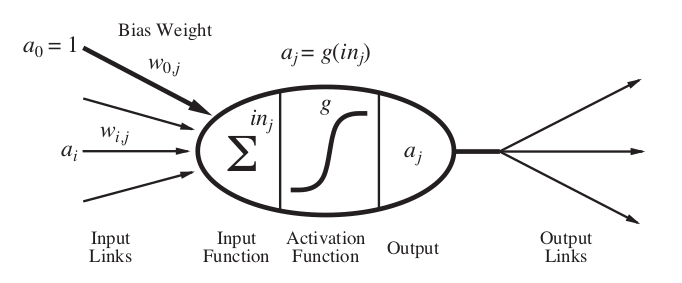
\includegraphics[width=0.8\linewidth]{img/perceptron.png}
    \caption{Model of the perceptron, taken from \cite[]{russell2016artificial}.}
    \label{fig:perceptron}
\end{figure}

A neural network is a collection of many of such neuron components, often layered. The properties of the neurons as well
as the overall network properties are called \emph{hyperparameters} and describe the overall architecture of the \ac{NN}.

A common architecture is the \emph{feed-forward network} which holds several layers of sets of neurons. Each set has no
connection within itself but its activation output is fed into the next layers neurons. It is therefore a directed
acyclic graph. Other than the weights, this network has no internal state and can therefore not hold information about
the input in some form of memory. An alternative is a \emph{\acl {RNN} } which includes loops and therefore can
hold state. The former network is often used for image classification problems while the latter is used for
time-series analysis and natural language processing.

When looking at \ac{NN} one important decision is the number of layers. In fact, the history of \acl{NN} has shown
three key phases of progress, the first phase which included simple single-layer networks, the second which included one
\emph{hidden layer} and the third phase, today, which uses networks that benefit of several hidden layers. A hidden
layer is a number of neurons between the input layer and the output layer. This allows the network to generate complex
input-output relationships. Such a multi-layer network is conceptualized in Figure~\ref{fig:multilayernn}. Each layer
$h^n$ feeds into the next until finally the output layer is reached.

\begin{figure}[]
    \centering
    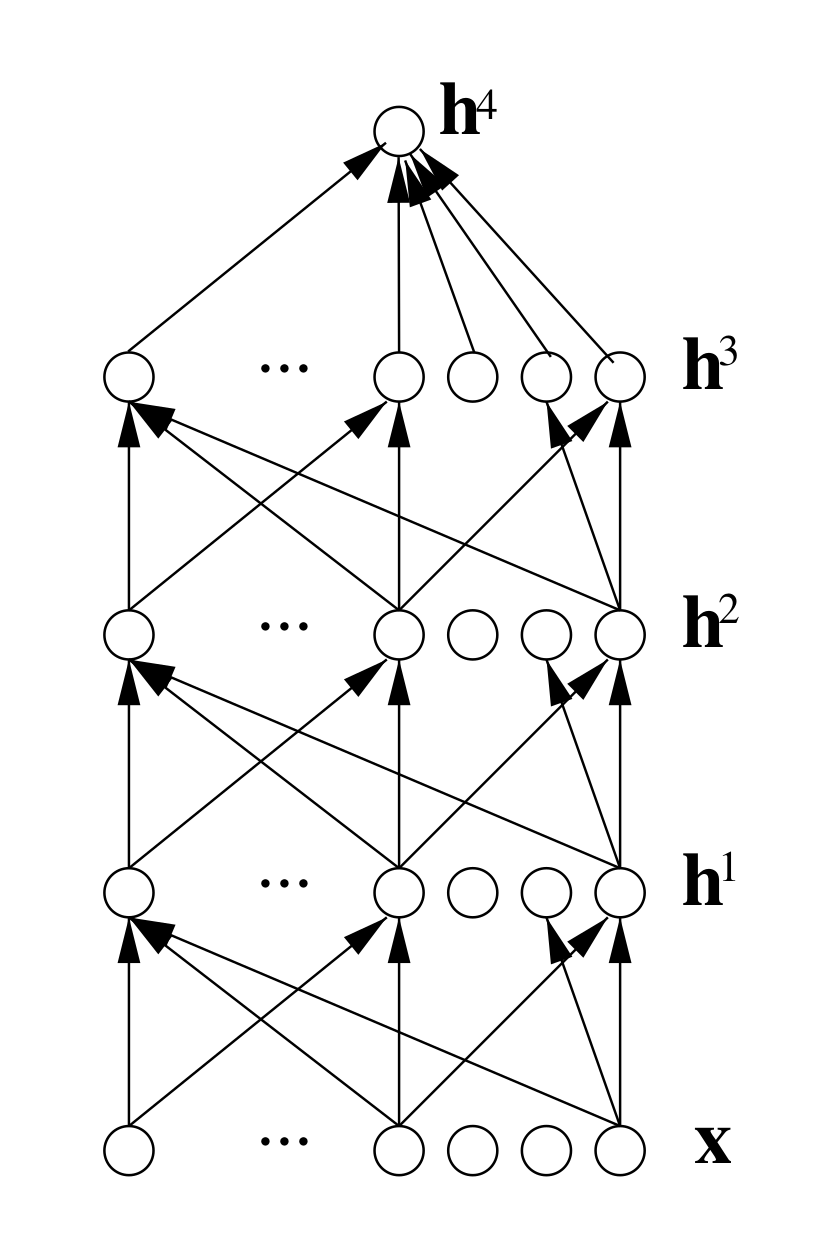
\includegraphics[width=0.3\linewidth]{img/multilayer_nn.png}
    \caption{Multi-layer neural network from \cite[]{bengio2009learning} }
    \label{fig:multilayernn}
\end{figure}

Neural networks can therefore represent complex non-linear and discontinuous functions
\cite[p.732]{russell2016artificial} even with small numbers of layers or neurons. Such \emph{deep} networks however long
suffered from a large issue: It was unclear how to train them, i.e. how to make them learn. The next section describes a
solution to this problem which lead to the latest revolution in \ac{NN} applications.

\subsection{Learning Neural Networks and Backpropagation}
\label{sec:Backpropagation}


%-------------------------------------------------------------------------------
% done unless professor adds notes
%-------------------------------------------------------------------------------


The previous sections have described learning in respect to the goal of the learning process and the input data that is
used to learn from. This section explains the forms of learning and focuses on one widely used form called
backpropagation.

When looking at \ac{NN} while remembering the definition of learning from earlier, it becomes clear that there are many
ways a \ac{NN} can change its state. It could:

\begin{enumerate}
    \item develop new connections
    \item remove existing connections
    \item change the connecting weights
    \item change the threshold values of the activation functions
    \item change its input function
    \item develop new neurons
    \item remove existing neurons \cite[p.60]{kriesel2007brief}
\end{enumerate}

Of these many actions, changing the weights is however the most common way to let a \ac{NN} learn. This is because many
of the other changes in its state can be performed by a specific way of changing the weights. Removing connections is
equivalent to setting the weight of the connection to 0 and forbidding further adaption afterwards. Equally, adding new
connections is the same as setting a weight of 0 to something that is not 0. Changing the theshold values can also be
achieved by modelling them as weights. Changing the input function is uncommon. The addition and removal of neurons
(i.e. the growing or shrinking of the network itself) is a popular field of research but will not be discussed further
\cite[p.60]{kriesel2007brief}.

Learning by changing the weights therefore covers a wide range of possible adaptions to the network structure. When
looking at a single (sigmoid) perceptron, the changing of the weights of its input values is the same process as that of the
concept of gradient descent algorithms. Because the activation function is most often \emph{soft}, to ensure
differentiability and because a hard threshold creates a non-continuous function, the process of fitting the weights to
minimize loss is called logistic regression \cite[p.729f.]{russell2016artificial}. For a detailed explanation of the gradient
descent approach, I will refer to the works of \citet{russell2016artificial} as well as
\citet{Goodfellow-et-al-2016}.



%logistic regression + gradient descent on a unit based view

The above described concept of learning from labeled examples is intuitive for single-layer \ac{NN}. The output can be
directly compared to the labels provided by the training set and logistic regression applied to correct the weights of
the network to reduce the loss. It becomes problematic though, when several layers are inserted between the input and
the output. The weights of the hidden layers are not included in the labeled examples. This is where the concept of
\emph{backpropagation} becomes useful. For Figure~\ref{fig:multilayernn}, any error of the weights of the neurons in
layer $h^1$ influence the values of the output values of layer $h^2$ and $h^3$ (in the case of fully connected layer).
For any additive loss function (such as $L_2$), the error however is simply the sum of the gradients of the losses of
the outputs\cite[p.733f.]{russell2016artificial}.

\begin{equation}
    \frac{\partial}{\partial w} Loss(w) =  \frac{\partial}{\partial w} \vert y-h_w(x) \vert ^2 = \frac{\partial}{\partial w} \sum_k{(y_k - a_k)^2} =  \sum_k{\frac{\partial}{\partial w}(y_k - a_k)^2}
    \label{equ:errorssum}
\end{equation}

where the index k ranges over nodes in the output layer \cite[p.733f.]{russell2016artificial}. This however does not
solve the issue that the training set doesn't include the expected values for the hidden layers. This is solved by
back-propagating the error values through the network. % TODO CONTINUE STOP

%network has e.g. 5 values in its output layer, each output depends on several of the previous layers activation values.  Therefore

\subsection{Recurrent Neural Networks}%
\label{sec:recurrent_neural_networks}

As was already noted in the previous chapter, \ac{NN} can be both acyclic and cyclic graphs. The
\emph{vanilla} \ac{NN} is usually considered to be an acyclic feed-forward network, as it has no internal state and is
therefore more suited to describe the concepts of how the networks operate. Especially in translation and text to speech
applications though, \ac{RNN} are popular as they are able to act on previously seen information in a sequence of
data. Generally they are suitable for many applications where the data has some kind of time-dependent embedding
\cite[p.373]{Goodfellow-et-al-2016}.

A \ac{RNN}, therefore computes its output based on the weights $w_i$, commonly noted as $\theta$, it's current input
$x^t$ and it's previous hidden units internal states $h^(t-1)$.

\[
    h^t = f(h^(t-1), x^t, \theta)
\]

The network generally learns to use $h^t$ to encode previously seen aspects relevant to the current task, although this
is inherently lossy as the previous number of inputs (i.e. $\mid t-1\mid$) is arbitrary. Figure~\ref{fig:rnn_concept}
shows this concept.

\begin{figure}[]
    \centering
    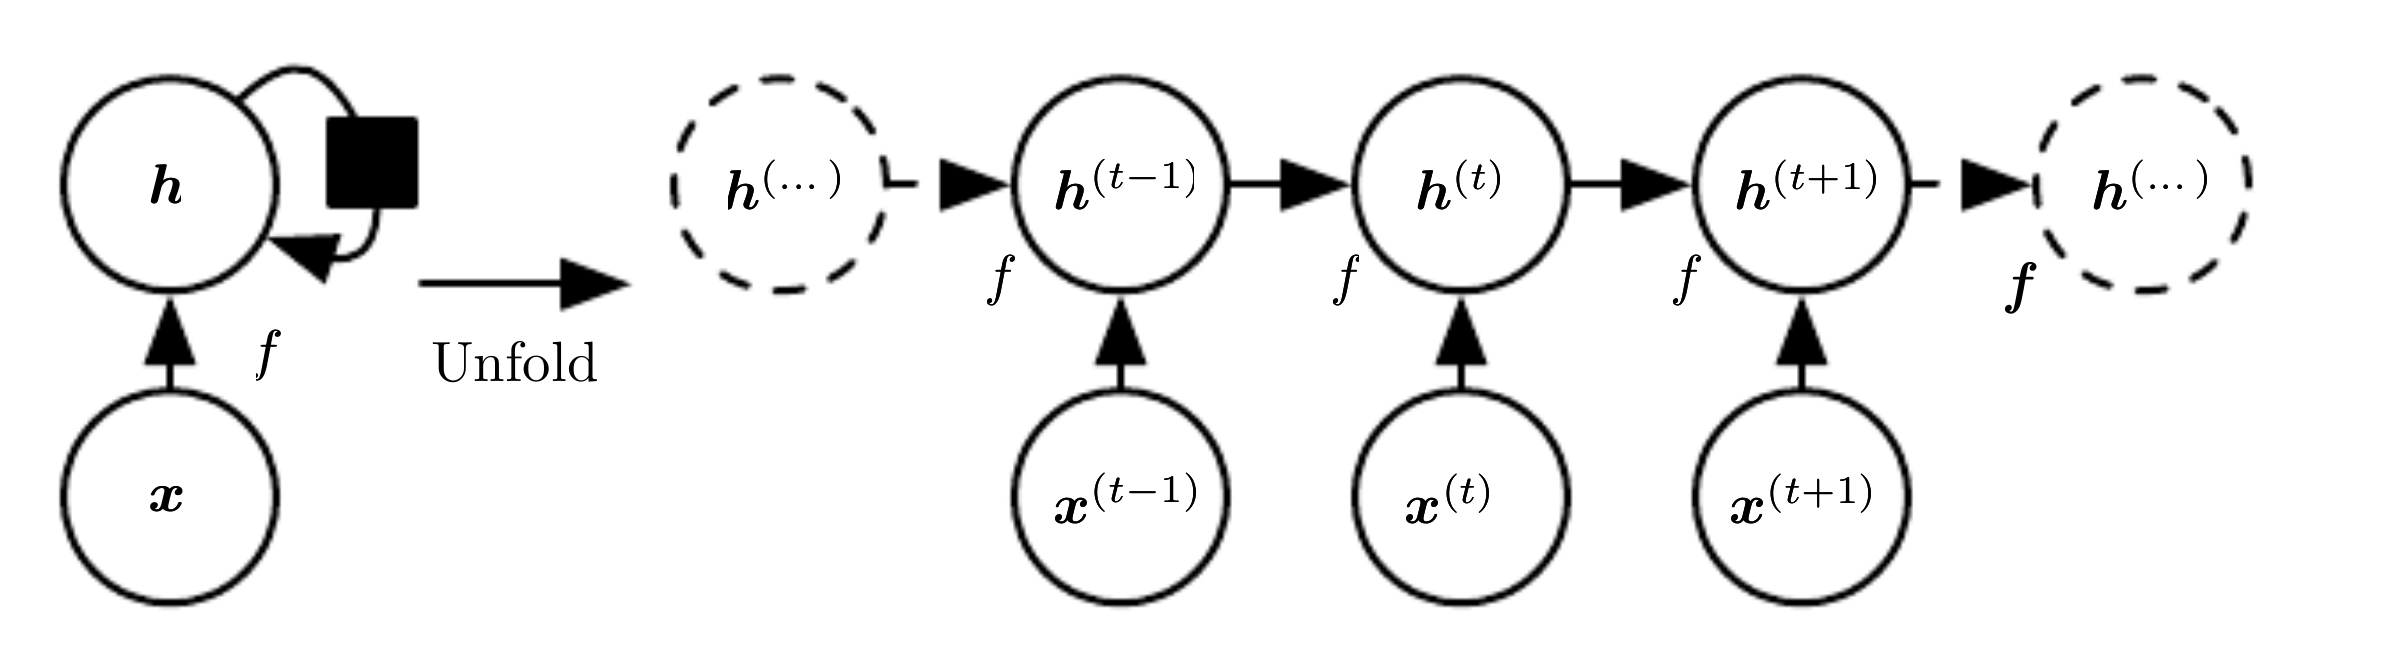
\includegraphics[width=0.8\linewidth]{img/rnn_concept.png}
    \caption[Recurrent Neural Network conceptualized]{. \emph{Left}: Circuit diagram where the black square represents a
        1 time slot delay. \emph{Right:} The same network unfolded where each node represents a particular time instance.
    Taken from \citet{Goodfellow-et-al-2016}.}
    \label{fig:rnn_concept}
\end{figure}

The network structure has two benefits: Firstly, it allows for arbitrary sequence length, as the network size is
dependent on the time slot specific input and not on the number of previous time slots. Secondly, the same network with
the same weights (or in mathematical terms the same transition function $f$) can be used during each time slot. This
means: When a \ac{RNN} is fed a sequence of data, the weights will stay the same throughout the sequence. They can be
updated after the entire sequence has been processed.

%TODO vanishing gradient problem and \ac{LSTM} GRU
Such recurrent systems, while theoretically able to hold information across inputs, suffer from an issue called the
\emph{vanishing gradient problem}. A network that sequentially processes 20 samples is not easily capable to hold useful
information within its state from the early beginning to then act upon it later in the sequence. This is a common
problem for translation: Sentences often have structures where the first word influences the meaning of the final one.
Th network processes each word at a time, quickly loosing the information that was inherent in the first word because it
is covered with noise from the other (potentially irrelevant) words. \citet{Hochreiter:1997:LSM:1246443.1246450}
developed he \ac{LSTM} model to solve this problem. Each unit in the network is actually a group of gates that act in
harmony to store information in a recurrent cell. \emph{Keep} gates allow the network to decide when the information in
the recurrent cell is supposed to be kept or discarded.
%TODO STOP --> write the gates needed for the recurrent cell stuff.


\section{Reinforcement Learning}

The previous chapters have introduced concepts of \ac{SL} , \ac{NN}, backpropagation and \ac{RNN} for time-embedded
learning tasks. \ac{RL} can be described as an intersection between supervised and unsupervised learning concepts and
Deep \ac{RL} is the usage of \ac{NN}, especially those with many layers, to perform \ac{RL}.

On the one hand \ac{RL}  does not require large amounts of labelled data to generate successful systems which is
beneficial for areas where such data is either expensive to aquire or difficult to clearly label. On the other hand it
requires some form of feedback. Generally, \ac{RL} \emph{agents} use feedback received from an \emph{environment}.  The
general principle of \ac{RL} therefore includes an agent and the environment in which it performs actions. The function
that determines the action $a$  taken by the agent in a given state $s$ is called its policy, usually represented by
$\pi$.  The environment reacts to the actions of the agent by returning new states $s'$ which are evaluated and a
corresponding reward $r$ is given to the agent. The reward gives the agent information about how well it performed
\citep[p.830f.]{russell2016artificial}.

%TODO still up to date with the following subsections?
This section will first introduce the concepts of a \ac{MDP}, then introduce different concepts of \ac{RL} agents,
describe approaches to encourage exploration of its options and finally describe how \ac{NN} can be used to create
state-of-the-art agents that can solve complex tasks. The majority of the chapter is based on
chapters 17 and 21 of \citet[]{russell2016artificial} unless otherwise marked.

\subsection{Markovian Decision Processes}%
\label{ssub:markovian_decision_processes}

A common model describing the conceptual process of states and actions followed by new states and new actions of an
agent and its environment is called a \acf {MDP}. In fact, \ac{RL} is an approach for solving such \ac{MDP} problems
optimally
\footnote{Although \ac{RL} can also be applied to non-sequential decision problems, the field has largely focused on
sequential problems}.

A \ac{MDP} is usually defined by the following components:

\begin{itemize}
    \item $\mathcal{A}$: Finite set of allowed actions
    \item $\mathcal{S}$: Finite set of states
    \item $P(s' \mid s,a) \forall s \in \mathcal{S}, a \in \mathcal{A}$: Probability of transitioning from state
        $s$ to state $s'$ when action $a$ is taken
    \item $\gamma$: Discount factor for each time slot, discounting future rewards to allow for long-term and
        short-term focus
    \item $R(s)$: Reward function that defines the reward received for transitioning into state $s$
\end{itemize}

To solve such a problem, an agent needs to be equipped with a policy $\pi$ that allows for corresponding actions to each
of the states. The type of policy can further be distinguished between \emph{stationary} and \emph{nonstationary}
policies. The former type refers to policies that recommend the same action for the same state independent of the
time step. The latter describes those policies which are trying to solve non-finite state spaces and where an
agent might therefore act differently once time becomes scarce. However, also infinite-horizon \ac{MDP} can have
terminal states which conceptually mean that the process has ended.

A more complex form of \ac{MDP} is the \ac{POMDP} which involves agents basing their actions on a belief of the
current state. As the later practical application to \ac{PowerTAC}  however can be mapped to a \ac{MDP}
where the transition probability implicitly represents the partial observability \citep{tactexurieli2016mdp}, this will not be discussed.

\subsection{Bellman Equation}%
\label{ssub:bellman_equation}

The Bellman Equation offers a way to describe the utility of each state in an \ac{MDP}. For this, it defines the
utility of a state as the reward for the current state plus the sum of all future rewards discounted by $\gamma$.

\begin{equation}
    U(s) = R(s) + \gamma \max_{a\in\mathcal{A}(s)} \sum_{s'}{P(s' \mid s,a)U(s')}
\end{equation}

In the above equation, the \emph{max} operation selects the optimal action in regard to all possible actions. The
Bellman equation is explicitly targeting \emph{discrete} state spaces. If the state transition graph is a cyclic graph
the solution to the Bellman equation requires some equation system solving. That is because $U(s')$ may depend on $U(s)$
and the other way around. Further, the \emph{max} operator creates nonlinearity which, for large state spaces, becomes
intractable quickly which is the reason for an iterative approach called \emph{Value Iteration}.

%In a discrete action space this would be a selection over all possible actions, in a continuous action space it however
%can become more complex. \ac{NN} based \ac{RL} agents simply invoke their policy network to retrieve the action which
%the agent believes it the one with the highest utility \citep{mnih2013playing}.


%As an example, an agent active in the environment of playing Super Mario may receive rewards corresponding to the game
%score. It may perform all valid moves permitted by the game and the goal is to improve its score.

%To train an agent, the task is usually performed several times and the environment is reset after each iteration to
%allow for a new learning step.
%TODO add atari games reference
%When thinking about such an agent, it becomes obvious that without some explicit incentive to explore new alternatives,
%it may be contempt with whatever success it achieves and then always perform the same action. To avoid this, the agent
%can either be forced to try new alternative actions (through forcing random actions in a certain percentage of cases) or
%through explicit rewards for random actions.
%\citep() %A3C TODO


%There are several forms of learning to solve a \ac{MDP} using \ac{RL} but for the purpose of this thesis I will focus
%on explaining how policy search algorithms work. Their goal is to find a good policy $\pi$ given a certain state $s$.
%Alternatives to this approach are concepts that try to learn expected future reward for future possible states, for
%available actions and others. %TODO not clean paragraph...

\subsection{Value and Policy Iteration}%
\label{sub:policy_and_value_iteration}

Value Iteration uses the Bellman equation to iteratively converge towards a correct estimation of each states utility,
assuming both the transition function $P(s' \ mid s,a) \forall s \in \mathcal{S}$ and the reward function $R(s)$ are
known to the agent.
In the algorithm, the utility of each state is updated based on the \emph{Bellman update} rule:
\begin{equation}
    U_{i+1}(s) \gets R(s) + \gamma \max_{a \in \mathcal{A}(s)} \sum_{s'}{P(s' \mid s,a) U_i(s')}
\end{equation}
This needs to be performed for \emph{each} state during \emph{each} iteration. It is clear how quickly this becomes
intractable as well when $\gamma$ is reasonably close to 1, meaning that also long-term rewards are taken into
consideration.

Practically, the agent however doesn't care much about the values of various states. It cares about making the right
decisions, using the value of states as a basis for doing so. It is often observed that the policy $\pi$ converges far
sooner than the utility estimates $U(s)$. This is the basis for the \emph{Policy Iteration} approach which alternates
between:
\begin{enumerate}
    \item evaluating the current policy $\pi_i$ by calculating $U_i=U^{\pi_i}$, the value of each state if $\pi$ is
        executed and
    \item improving the policy using one-step look-ahead based on $U_i$
\end{enumerate}

This process stops when the policy is no longer showing any significant improvements in respect to its loss value. It is
generally also not necessary to always apply the above operations to \emph{every} state. Instead, state values and
policies can be updated only in respect to newly discovered knowledge regarding specific states or specific actions.
This is called \emph{asynchronous policy iteration}.

Both variants require the transition function and the reward function to be known to the agent. \ac{RL} research has
developed several methods that adapt the concepts of the two iteration algorithms for environments with the two unknown
functions. They are explained in the next sections.
%It allows for many interesting concepts to be used such as distributed learning, using multiple agents to explore an
%environment and learn from all their observations centrally, and

\subsection{Temporal Difference Learning}%
\label{sub:temporal_difference_learning}

When the underlying transition function is not known, but the agent has the ability to perform many trial runs in the
environment, an empirical approach can be adapted. For this, the agent performs a number of trials where it acts
according to a (fixed) policy and observes the rewards it receives. Each string of alternating actions and observations
is called a trial
\footnote{in newer \ac{RL} literature this is also called a \emph{trajectory} \citep{proximalpolicyopt, heess2017emergence} }.
The update rule for the utility of each state is as follows:
\begin{equation}
    U^\pi(s) \gets U^\pi(s) + \alpha(R(s) + \gamma U^\pi(s') - U^\pi(s))
\end{equation}
Where $\alpha$ is the learning rate and $U^\pi$ the utility under the execution of $\pi(s)$ in state $s$. This only
updates the utilities based on the observed transitions so if the unknown transition function sometimes leads to
extremely negative rewards through rare transitions, this is unlikely to be captured. However, with sufficiently many
trials, these rare probabilities will be adequately represented in the utilities for the states. If $\alpha$ is
continuously reduced appropriately, this will converge to the correct value.

\subsection{Exploration}%
\label{sub:exploration}

The above learning approach has one weakness: It is only based on observed utilities. If $\pi$ follows the pattern of
always choosing the action that leads to the highest expected $U_{i+1}$, i.e.
\begin{equation}
    \pi(s) = \max_{a \in \mathcal{A}(s)}P(s' \mid s, a)U(s')
\end{equation}
then it will never explore possible alternatives and will very quickly get stuck on a rigid action
pattern mapping each state to a resulting action. To avoid this, the concept of \emph{exploration} has been introduced.
There are many approaches to encourage exploration. The simplest is to define a factor $\epsilon$ which defines the
probability of choosing a random action at each step.
A more advanced variant is to add a term to the loss function that
corresponds to negative entropy of the policy $-\beta H(\pi(a \mid s ))$ where $H$ measures the entropy of a series of
actions. This encourages randomness in the policy but it permits the policy function to determine how this randomness
gets to occur \citep{schmitt2018kickstarting}. This entropy based loss also automatically regulates itself: When the
agent is not at all capable of choosing rewarding actions it reduces its loss through high entropy choices, i.e. lots of
exploration. Once the agent finds actions for certain states that lead to high rewards, choosing other random actions
negatively outweighs following the best action. Therefore, it becomes less random and the entropy reduces. If $\beta$ is
progressively lowered, the impact on the loss is also progressively lowered, allowing the agent to continuously improve
its loss despite less exploration.
Another alternative is the positive weighting of actions in states that have not been tried yet, essentially giving such
actions an optimistic prior as if they promise higher rewards than the already explored regions. This is easy to
implement for small, discrete state and action spaces but more complex for continuous spaces.

% Q Learning and Deep-Q learning
% Policy Gradient


%\subsection{Policy Search}
%\subsection{Deep Reinforcement Learning}
%%TODO paper deep \ac{RL} > mixing R.L and deep \ac{NN}
%\subsection{Proximal Policy Optimization OR(TBD) Deep Q learning}
\subsection{Q Learning}%
\label{sub:q_learning}

In Section~\ref{sub:policy_and_value_iteration} I have already described how to learn the values of states, given an
action. This action can also be derived from a policy function.  In the case of an agent that wants to learn its policy
(i.e. learn what a good policy is), this becomes problematic if the transition function is not known. An alternative
model is called \emph{Q-Learning} which is a form of Temporal Difference Learning. It learns an action-utility value
instead of simply the values. The relationship between this \emph{Q-Value} and the former value of a state is simply
\begin{equation}
    U(s) = \max_{a}Q(s,a)
\end{equation}
so the value of a state is that of the highest Q-Value. The benefit of this approach is that it does not require a model
of how the world works, it therefore is called a \emph{model-free} method. The update rule for the Q-Values is simply
the Bellman equation with $U(s)$ and $U(s')$ replaced with $Q(s,a)$ and $Q(s',a')$ respectively.

The update rules for the Q-Value approach are related to the Temporal Difference Learning rules but include a $\max$
operator
\begin{equation}
    Q(s,a) \gets Q(s,a) + \alpha(R(s) + \gamma \max_{a'}Q(s', a') - Q(s,a))
\end{equation}
An alternative version is the reduction of the above equation by removing the $\max$ operator. This results in the
\emph{actual} action being considered instead of the one that the policy believes to be the best. Q-Learning is
\emph{off-policy} while the latter version, called \ac{SARSA}, is \emph{on-policy}. The distinction has a significant
consequence: While Q-Learning may be used to learn the Q-Values from recorded state-action pairs, \ac{SARSA} requires
the action taken to be derived from the current policy function.

\subsection{Policy Search and Policy Gradient Methods}%
\label{sub:policy_search_and_policy_gradient_methods}

These two approaches are possibly the simplest of the \ac{RL} algorithms. In its simplest form, policy search requires
the algorithm to start with an initial policy and then adapt this policy until no further gains can be made. While the
concepts is simple, it may lead to significant performances, if the \emph{choices regarding what to change} are made
wisely. If the policy is just randomly changed, the results will be equally random. If the policy is changed depending
on a good interpretation of the environments responses however, this method can offer good performance without the need
to have a model of how the world works. Such an agent simply takes the current state $s$ as input and uses its policy to
determine an output action $a = \pi(s)$. The value of a policy is noted as $\rho(\theta)$.

For simplicity, I will assume actions derived from a policy to be continuous as both the later application relies on
such actions and because the analysis of policy search algorithms becomes more complex in discrete action spaces. When
both the policy and the environment are deterministic and without noise, policy search algorithms are actually extremely
effective. The agent can repeat actions in the equivalent states several times, adapting its policy parameters $\theta$ by
small values and determine the empirical gradient values which allow the agent to perform hill-climbing in the policy
function. This will converge to a local optimum, hence simply trying different actions allows the agent to improve its
performance as long as the local optimum has not been reached.

In real world scenarios however, environments (and also policies) are commonly stochastic. Changing the policy
parameters $\theta$ by a very small value and comparing results of two instances of executing the policy may lead to
strong variations in the reward due to the stochasticity of the environment and therefore the noise in the reward
signal. This is a common problem of statistics and the typical answer is to increase the number of trials until
statistical significance can be reached. But this is often impractical for real world problems and also not the best
approach.

The general idea of modern policy gradient methods therefore follows an approach of using a different function as an
estimator for the gradient of the policy in a given configuration. A common approach is to use an advantage function
$\hat{A}_t$ to create an estimator for the policy gradient:


\begin{equation}
    \hat{g} \ =\ \hat{\mathbb{E}}_{t} \ \left[ \nabla _{\theta }\log \pi _{\theta }( a_{t} \ \mid s_{t})\hat{A}_{t}  \right]
\end{equation}

where $\hat{A}_t$ describes the advantage of taking one action over another in a given state. It can therefore be
described as an \emph{actor-critic architecture}, because $A(a_t, s_t) = Q(a_t,s_t) - V(s_t)$, meaning that the
advantage value is equivalent to the difference in the estimated value of the state itself and the value of performing
a specific action (derived from the policy) in that state \citep{mnih2016asynchronous}

\subsection{Deep Learning in Reinforcement Settings}%
\label{sub:deep_learning_in_reinforcement_settings}

The previous sections have outlined the conceptual approaches for designing learning agents based on various approaches
for what is essentially a system that tries to act intelligently in respect to its environment. Especially in recent
years, many breakthroughs have been driven by using \ac{NN} in \ac{RL} settings. \ac{NN} have proven effective as
parameterized Q-Value estimators, state-value estimators and as policy functions. Most approaches suffer similar
problems: Data efficiency in respect to the trial number required to learn a desired skill, scalability and robustness
\citep{proximalpolicyopt}. The reasons for these challenges are obvious: The agents receives minimal feedback and it has
a hard time mapping its received reward to specific alterations in its behavior (aka credit assignment problem)
\citep{arulkumaran2017brief}.

The research has shown many approaches to alleviate these shortcomings: Inverse Reinforcement Learning allows the
learning of a policy by imitating a trusted expert, allowing faster learning rates through clear signals
\citep{NG2000InvReinf}. \citet{brockman2016openai} have created the \emph{gym} which allows for coherent benchmarking of
various approaches against a common set of challenges. \citet{hafner2017agents} have created a setup that allows for
massive parallel processing of several environments which all contribute to the improvement of a central policy
function. The implemented algorithm uses \ac{NN} and an advanced form of the advantage based policy methods introduced
earlier. By this time, the research groups were usually referring to their agents learning progress in the range of
millions of time slots \citep{proximalpolicyopt}. One common argument for the benefit of \ac{AI} is the ability to
transfer knowledge learned by one agent to many agents. The structure of \ac{NN} however makes it difficult to transfer
knowledge between agents with varying hyperparameters. The weights for the neurons cannot simply be copied between
networks with different structures and due to the complexity of the systems, learning them again from scratch is
resource intensive.

\citet{matiisen2017teacher} have introduced a concept that helps agents learn faster by breaking complex challenges down
into several simpler sub tasks, similar to how humans are taught in educational institutes. This allows researchers to
quickly get new generations of agents up to speed with their predecessors.

Another approach to solve this problem of repetitive learning has been introduced by \citet{schmitt2018kickstarting}. In
their setup, the newly created agent transitions from trying to act similar as its \emph{teacher agent} towards trying
to improve its performance independently. To achieve this, the student agent includes a term that describes the
difference between its action and the action its teacher would have taken.

In summary, many tweaks to the core concepts allow for improvements in the challenges outlined before. Faster learning given limited
ressources through bootstrapping, improving wall time by leveraging large-scale architectures through and
parallelization, transfering knowledge from (human) experts through inverse \ac{RL} etc. A rich landscape of tools is
in rapid development and to construct an effective agent, it is important to leverage both the specific problem domain
structure and the available resources.

%TODO still needed after paper by DeepMind? --> showed that learning from teacher helps

%\section{Competitive Simulations}%as a tool of experimental research into AI

\section{PowerTAC: A Competitive Simulation}%
\label{sec:powertac_a_competitive_simulation}



%TODO alternative sources / implementations like powertac
% Simulating the effect on the energy efficiency of smart grid technologies.pdf
In the following chapter, I will introduce the \acl{PowerTAC}. It's simulating a liberalized retail electrical energy
market where multiple autonomous agents compete in different markets. Firstly, a retail market where agents, or
\emph{brokers}, compete for numerous end-users through the offering of tariff contracts. Secondly, a wholesale market in
which brokers buy and sell large amounts of electric energy to match their customers demands. This market allows brokers
to place bids up to 24 hours in advance and each hour the broker has the ability to place new bids to correct for
changes in their forecast models. Lastly, the balancing market which places relatively high costs on any broker that
causes an imbalance in the system, giving incentives to the brokers to balance their own portfolios prior to the
balancing operations. Figure ~\ref{fig:powertacoverview} summarizes this ecosystem.

%TODO have i also explained how the brokers get punished for peaks etc? what about the accounting models.

\begin{figure}[!h]%!h \centering
    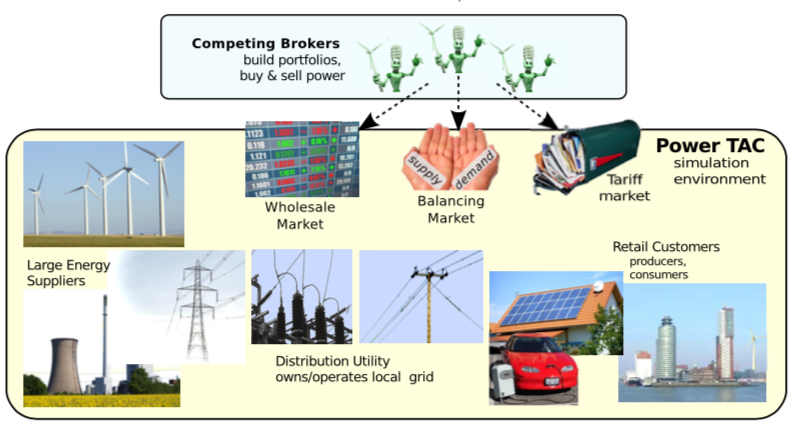
\includegraphics[width=0.9\textwidth]{powerTACScenarioOverview.png} \caption{PowerTAC overview of markets}
\label{fig:powertacoverview} \end{figure}


%OVERVIEW,Economical
The broker to be developed has to contest in a number of markets and handle a variety of customer types. While
\ac{PowerTAC} generates a fairly complex landscape, it mostly aims at economic complexity rather than
modeling the technical underpinnings of the system. It therefore doesn't simulate any hardware but rather focuses on the
different agents involved in the market.

%TIMESLOTS
The simulation emulates a time span of approximately 60 days with 1h time slot precision and accelerates this to 5
real-world seconds corresponding to each game-hour. The simulation emulates a time span of approximately 60 days with 1h
time slot precision and accelerates this to 5 real-world seconds corresponding to each game-hour.


\subsection{Components}%
\label{sub:components}



The simulation is both technically and logically separated into several components to aid both comprehensibility of the
system and yet allow complex simulations of more realistic scenarios. In the following pages, those logical components
will be explained. Most of these components are easily mappable into the technical implementation.

\subsubsection{Distribution Utility} The \ac{DU} represents an entity that regulates the real-time electric usage and
corrects for any imbalances in brokers portfolios by correcting the overall net-balance of the system. Any broker who
did not balance it's electric supply and demand incurs costs and is therefore incentivized to always balance its
portfolios as good as possible. It also owns the distribution grid and every broker must pay fees for the use of the
grid in proportion to the number of the customers it serves \citep[p.10]{ketter2018powertac}. It also offers tariffs and
is therefore the equivalent of a \emph{baseline broker} whose tariffs create an upper bound on broker profitability.

\subsubsection{Accounting} All accounting is managed by the central simulation server as to avoid adversarial brokers
from tampering with the games rules. Negative balances are usually punished with a 10\% p.a. interest rate while
positive balances receive a 5\% p.a. interest rate. This components tracks every brokers financial balance as well as
all brokers customer subscriptions and wholesale market positions \citep[p.11]{ketter2018powertac}.

\subsubsection{Wholesale Market}
%TODO energy or electricity? What's the "right" word? --> ENERGY
Every broker needs to purchase energy before it can sell it to the customers unless the customers of the broker itself
generate sufficient energy to balance its own portfolio. For this, \ac{PowerTAC} offers a wholesale market that operates
a \emph{periodic double auction} which represents traditional energy exchanges like those existing in the United States
and European markets. Participants in this wholesale market are all brokers as well as a large general entity
representing a number of generating facilities, a grid buyer who simulates large-scale demands based on real-world data
adjusted based on weather-forecasts and a wholesale buyer who regularly places high-volume, low-price bids. During each
time slot, 24 future slots are open for placing bids by the brokers. After the bids have been collected, a clearing
price gets calculated which is the intersection between the supply and demand curves. Orders without limit prices are
always served first. After the clearing, all uncleared bids and asks are distributed to the brokers to indicate the
direction of the markets' demand and supply curves.

\subsubsection{Balancing Market} The Balancing market is the last and final trading opportunity for agents and in the
sense of the game is at $t-0$ meaning that it occurs virtually in parallel to the consume of electricity. Any imbalance
during this phase gets corrected for by the \ac{DU} who imposes forced balancing of brokers with an imbalanced
portfolio. Brokers with too much supply in their portfolio therefore receive very little reimbursement for it and those
whose customers' usage is higher than the estimated amount pay high prices for the additionally supplied energy.

Brokers who have tariffs with economic control abilities can pass this capacity along to the \ac{DU} who utilizes these
capacities to correct the markets imbalances, charging customers' storage devices if an oversupply is present or
depleting their devices in the case of an under-supply. It is therefore economically beneficial for brokers to attract
customers with such balancing capabilities since it offers a buffer capacity against the balancing costs otherwise
incurred through the actions of the \ac{DU} \citep[p.5]{ketter2018powertac} .





\subsubsection{Customer Market}

The foundation for any broker making profit is a sufficient amount of customers being subscribed to its tariffs. For
this to occur, the broker must publish tariffs that are competitive as to attract customers. On the other hand, if the
broker offers tariffs that lead to net losses, long term profit will not be possible
\footnote{While the 2017
    competition technically allowed for brokers to remain in the game despite offering highly under priced tariffs that
    corrupted the simulation results, a proper broker must not pursue such strategies simply because of economical
reasoning.}

The broker has a wide variety of actions at its disposal to create a rich portfolio. The simulation offers the
creation of a variety of tariff types that have variables which are adaptable by the broker. The types include:

\begin{description}
    \item[Flat rate] Customers pay a flat rate per kWh and they always receive their demanded
        amount.
    \item[Tariff with fixed fee] Customers pay a definable fixed fee every day to receive the service.
    \item [Tiered rates] Customers pay a certain price per kWh until a limit is reached after which the kWh price
        changes.  Arbitrarily many such tiers can be added.  \item[Time-of-use] Customers pay different prices depending
        on the time of the day or the day of the week.  \item[Dyanmic Pricing] Allows the broker to dynamically adapt
        the price per kWh in real-time to incentives customers to reduce their usage during high demand times. A
        minimum, maximum and mean price per kWh as well as a notification interval needs to be specified.
    \item[Curtailable] Customers can opt in to a tariff that allows the broker to reduce the delivered amount of
        electricity per time slot up to a certain percentage. This means the customer is exposed to a risk of not
        receiving the entire electrical supply demanded, usually for a discounted unit cost per kWh.  \item[Storage]
        Customers can offer their storage capacity to brokers to allow the broker to balance his portfolio. Customers
        receive payment from the broker if their storage devices are being depleted and pay a (reduced) fee for charging
        events \citep[p.9]{ketter2018powertac}.
    \item[Signup fees and withdrawl fees] Customers can receive bonuses or pay fees
        for signing up or canceling a subscription.
\end{description}

Some of the above types can also be combined to create complex tariff landscapes for customers to choose from.

\subsubsection{Customer models}% \label{sub:customer_models}

The final part of the simulation environment is made up by the customer models which simulate real-world customers.
Each customer can both produce and consume electricity. Consumers are modeled both by factored and elemental models
\citep[p.14]{ketter2018powertac}, allowing for small numbers but detailed patterns and large number averaged
patterns respectively. The customers evaluate the offered tariffs based on a number of deterministic functions
including the various costs and variants of the offered tariffs multiplied by a \emph{irrationality factor} that
allows for a more realistic limited rationality of the actors. Additional assessments such as broker reputation
evaluation and energy source preferences are also included in the utility function.

Customers do not evaluate every new tariff but only do so irregularly based on an \emph{inertia factor} that limits
their attention to new tariffs. Customers are not inherently loyal to their brokers but the inertia factor
indirectly causes customers to not immediately switch if there is a more rational tariff available.

As previously noted, customers can both consume and produce electricity. While most production is non deterministic
and non controllable (i.e. in the case of solar and wind electricity), some are controllable such as \ac{CHP} or
bio-gas units \citep[p.16]{ketter2018powertac}. Devices such as electric vehicles or water heaters can also offer
regulation actions to brokers to balance their portfolios. A \emph{smart} water heater could refill only minimally
after heavy use if usage patterns show that the owners will most likely not use it again for several hours. This
way, an additional capacity for energy consumption is created that can be profitable for the customer, as the broker
usually charges less for electricity delivered under capacity regulation terms \citep[p.14ff.]{ketter2018powertac}.

\subsection{Applying observation learning to PowerTAC}%
\label{sub:applying_observation_learning_to_powertac}

In this section I describe some concepts that may be pursued in the development of more performant brokers for
\ac{PowerTAC}. They all adhere to the idea to learn from either previously recorded actions of other brokers or by
observing other brokers in the environment.

Generally, a neural network based policy function or value function requires
a significant amount of training. Similarly, supervised learning problems require a large training dataset to converge
onto their potential performance. Running a simulation takes about 3 hours and delivers some 1600 training steps. This
is far below what supervised learning algorithms can train on in a given time span and also \ac{RL} agent algorithms can
perform several hundred steps a second on contemporary hardware. When accelerating the training of the network using
modern \ac{GPU}s, this discrepancy becomes even more significant. For the \ac{RL} based wholesale trading component,
some techniques can be applied to boost its learning performance prior to having it interact with a live environment.
These techniques are described below

\subsubsection{Offline record based wholesale environment approximation}%
\label{ssub:offline_record_based_wholesale_environment_approximation}

\ac{PowerTAC} allows developers to download large amounts of historical game records. Several hundred games are
available for 2017 alone, ranging in number of competing brokers to simulate different market settings. The
\texttt{powertac-tools} repository makes it convenient to download all  of them and analyze them for specific data,
providng csv files for further analysis. I created records for all games downloadable for 2017 to let the broker train on
the datasets. For the wholesale trader, two data types are of interest initially, although further data may be provided
to improve the algorithms performance. The customer usage analysis
\footnote{\texttt{CustomerProductionConsumption.java}}
provides a historical dataset to create a
hypothetical portfolio for the learning \ac{RL} agent. To design a \ac{RL} environment, the broker needs a realistic
portfolio of required energy. Therefore, a subset of the customers may be choosen to pose as the brokers portfolio.
While in a real simulation setting, the customers constantly join and leave brokers tariffs, this offline environment
approximation assumes a static portfolio. Furthermore, the marketprices analysis
\footnote{\texttt{MktPriceStats.java}} gives a historical record of all market closings for each game. In this
environment approximation, the market prices don't get influenced by the brokers placement of ask or bid orders. This is
unrealistic if the broker represents any significant percentage of the overall market but may be a good approximation if
the portfolio of the broker is only covering a small percentage of the market. Ultimately, this environment allows for
rapid training of a \ac{RL} agent in the \ac{PowerTAC} environment by approximating its wholesale market. This is
because the agent is in control of the step flow, meaning it triggers the next time slot when it has completed its
actions instead of having to wait for the server to inform it about a new open time slot.

\subsubsection{Learning from historical actions of teacher agents}%
\label{ssub:learning_from_historical_actions_of_teacher_agents}

The \ac{RL} agent may in addition to a fixed portfolio be taught to imitate the recorded behavior of a teacher broker
such as a former winner of the competition. It may be given the recorded demand data of a competing broker and the
reward function would be modeled in a way that incentivizes the agent to behave similar to its teacher broker. This is
in accordance to the concepts of inverse reinforcement learning. If the broker may also act in a live competition, it
could implement the kickstarting concept of \citet{schmitt2018kickstarting}, feeding its observations to a competitor
teacher broker and initially attempt to align its actions to those of the teaching broker. Unfortunately, this concept is difficult to
implement in the \ac{PowerTAC} environment. Brokers are black boxes and it is not possible to assume that they will
behave correctly if their submitted actions are not the actions that are actually submitted to the server. This would be
required, because the learning agent is the one that actually determines the policy, only giving its observations to the
teacher agent to \emph{ask for its opinion}. \citet{schmitt2018kickstarting} model lets the agent consider the question
of what its teacher would do if it were in its situation. Due to the inaccessibility of the teaching brokers inner
workings, an alternative model could only ask \emph{what would I do if I were in my teachers situation}. To allow for
such analysis, the next technique is required.

\subsubsection{Counterfactual analysis}%
\label{ssub:counterfactual_analysis}

Many real-world problems are approachable with \ac{RL} agent research. What makes \ac{PowerTAC} and other simulations
interestig is the ability to perform counterfactual steps. A counterfactual event is one that is not aligned with what
is actually true. In a real scenario, the phrase \emph{"Alan Turing would have not solved the Enigma encryption if he
had been fed one apple a day by his mother every morning"} is against what is actually true and therefore cannot
possibly be verified. In the \ac{PowerTAC} simulation, this is very different. Because the entire state of the server is
recorded in its state files, it can be reproduced exactly. Unfortunately, the brokers do not offer such ability to
reproduce their state. A level of randomness is inherent in their decision making. If a statement were to be: \emph{"Had
the broker offered tariff X in timestep 1200, it would have won the competition"}, it is not possible to reproduce the
state of the server from the state files alone to verify this hypothesis.

With a technology that allows for \emph{snapshotting} of memory space in Linux, it is possible to create a snapshot of
the server state and all its participants running on the same machine. A broker developer may therefore include the
ability to create a snapshot of the entire environment state to evaluate a number of alternative actions at any point
within the game instead of having to rerun an entire simulation. This means, a \ac{RL} agent can learn not simply
through performing full episodes within a learning session, slightly altering its behavior randomly within each episode.
If the network can determine points within a \ac{MDP} where a number of actions are available and any one may lead to an
increase in future rewards, the agent may decide to try all or a subset of the possible actions to determine which of
the alternative actions leads to the highest rewards. The concept would therefore be a bit different from usual \ac{MDP}
models. It would allow the agent to submit a range of actions and ask the environment to give back a range of
alternative scenarios and rewards. While this is still susceptible to random behavior \emph{after} the snapshot occured,
it is guaranteed to be the exact same state at the point where multiple actions are considered. Remaining uncertainty
may now be compensated by running a significant amount of trials ceteris paribus.

%TODO graphic



\subsection{Existing broker concepts}%
\label{sub:existing_broker_concepts}
Before designing my own agent, it is obvious to investigate previously developed agents and their design to understand
the current state of research. For this, I have analyzed the papers of the AgentUDE, TacTex and COLDPower, as they
performed well in previous tournaments. Their architectures, models and performances are summarized in the following
sections.




\subsubsection{Decision areas}%
\label{ssub:decision_areas}



\subsubsection{Decision models}%
\label{ssub:decision_models}

\subsubsection{Past performances}%
\label{ssub:past_performances}


\chapter{Implementation}

The following chapter will describe the concepts and reasons behind various components needed to allow a broker to
leverage modern reinforcement learning tools and algorithm libraries in the \ac{PowerTAC} environment. Current state-of-the-art
algorithms for \ac{RL}, available mostly in Python \citep{baselines}, are used. These leverage both the TensorFlow and
Keras high-level abstraction library \citep{plappert2016kerasrl}.

%TODO what-if yes or no... make a choice dude
%In general, a considerable amount of work was invested enabling communication between an agent
%written in Python and the \ac{PowerTAC} systems which are Java based. The preliminary research and its results are summarized in
%Section~\ref{sec:connecting_python_agents_to_powertac}. Because of this additional complexity, the practical part of the thesis was
%restructured to allow for successful contribution to the \ac{RL} field by performing a form of \emph{what-if}
%analysis in the wholesale market which is described in Section~\ref{sub:wholesale_market}. The Python environment has
%been constructed in a way to allow for future developers to leverage it as a framework for developing a fully capable
%agent that acts in all markets.

The overall architecture of the broker is composed of 5 main components: The communication abstraction, wholesale market
agent, balancing market agent, tariff market agent and demand predictor. In this implementation, only the wholesale
market and demand predictor are actively making decisions. Future researchers can make use of the component structure however.
The architecture is visualized in Figure~\ref{fig:agentframework}.

While \citep{tactexurieli2016mdp} have defined the entire simulation as a \ac{POMDP} (although they interpret it as a
\ac{MDP} for ease of implementation) with all three markets integrated into one problem, I believe breaking the problem
into distinct sub-problems is a better approach as each of them can be looked at in separation and a learning algorithm
can be applied to improve performance without needing to consider potentially other areas of decision making. A
subsequent algorithm could then be trained to perform the same actions as one unified decision making system according
to the concepts of \emph{Curriculum Learning}\citep{matiisen2017teacher} and \emph{Transfer Learning}
\citep{parisotto2015actor}. Such steps require more advanced forms of machine learning architectures and should
therefore be approached in future work.
To justify this separation of concerns, I refer to the estimation of fitness for a given tariff in a given environment.
A tariffs' competitiveness in a given environment is independent of the wholesale or balancing trading strategy of the
agent since the customers do not care about the profitability of the agent or how often it receives balancing penalties.
While the broker might incur large losses if a tariff is too competitive (by offering prices that are below the
profitability line of the broker), such a tariff would theoretically be quiet competitive and should therefore be rated
as such. The question which of the tariffs to actually offer on the market is a separate problem, that balances
competitiveness against profitability. Similar arguments can be made for the other components.

I will first describe a number of tools used in the implementation as well as the preprocessing of the existing data
using both new and existing code. Afterwards I will describe the new communication architecture for non-java clients.
Finally I will explain the code behind the two implemented learning components, the demand prediction and the wholesale
trading agent.

%The overall architecture for the agent is composed of three key modules.First, the environment module, which hosts all known
%information about the environment of the broker. This is used by all learning components. Second, A communication module
%bridges the environment module and the \ac{PowerTAC} environment to hide communication overhead from the agent code,
%letting the learning components access the environment as if it was not remotely defined.
%Third, the agent components module holds all learning components such as the wholesale trader, the demand estimator
%and the tariff manager. In the scope of this thesis, only the demand estimator and the wholesale trader were implemented
%but the framework allows for the additional components to be easily implemented. The architecture is visualized in
%Figure~\ref{fig:agentframework}.

\begin{figure}[]
    \centering
    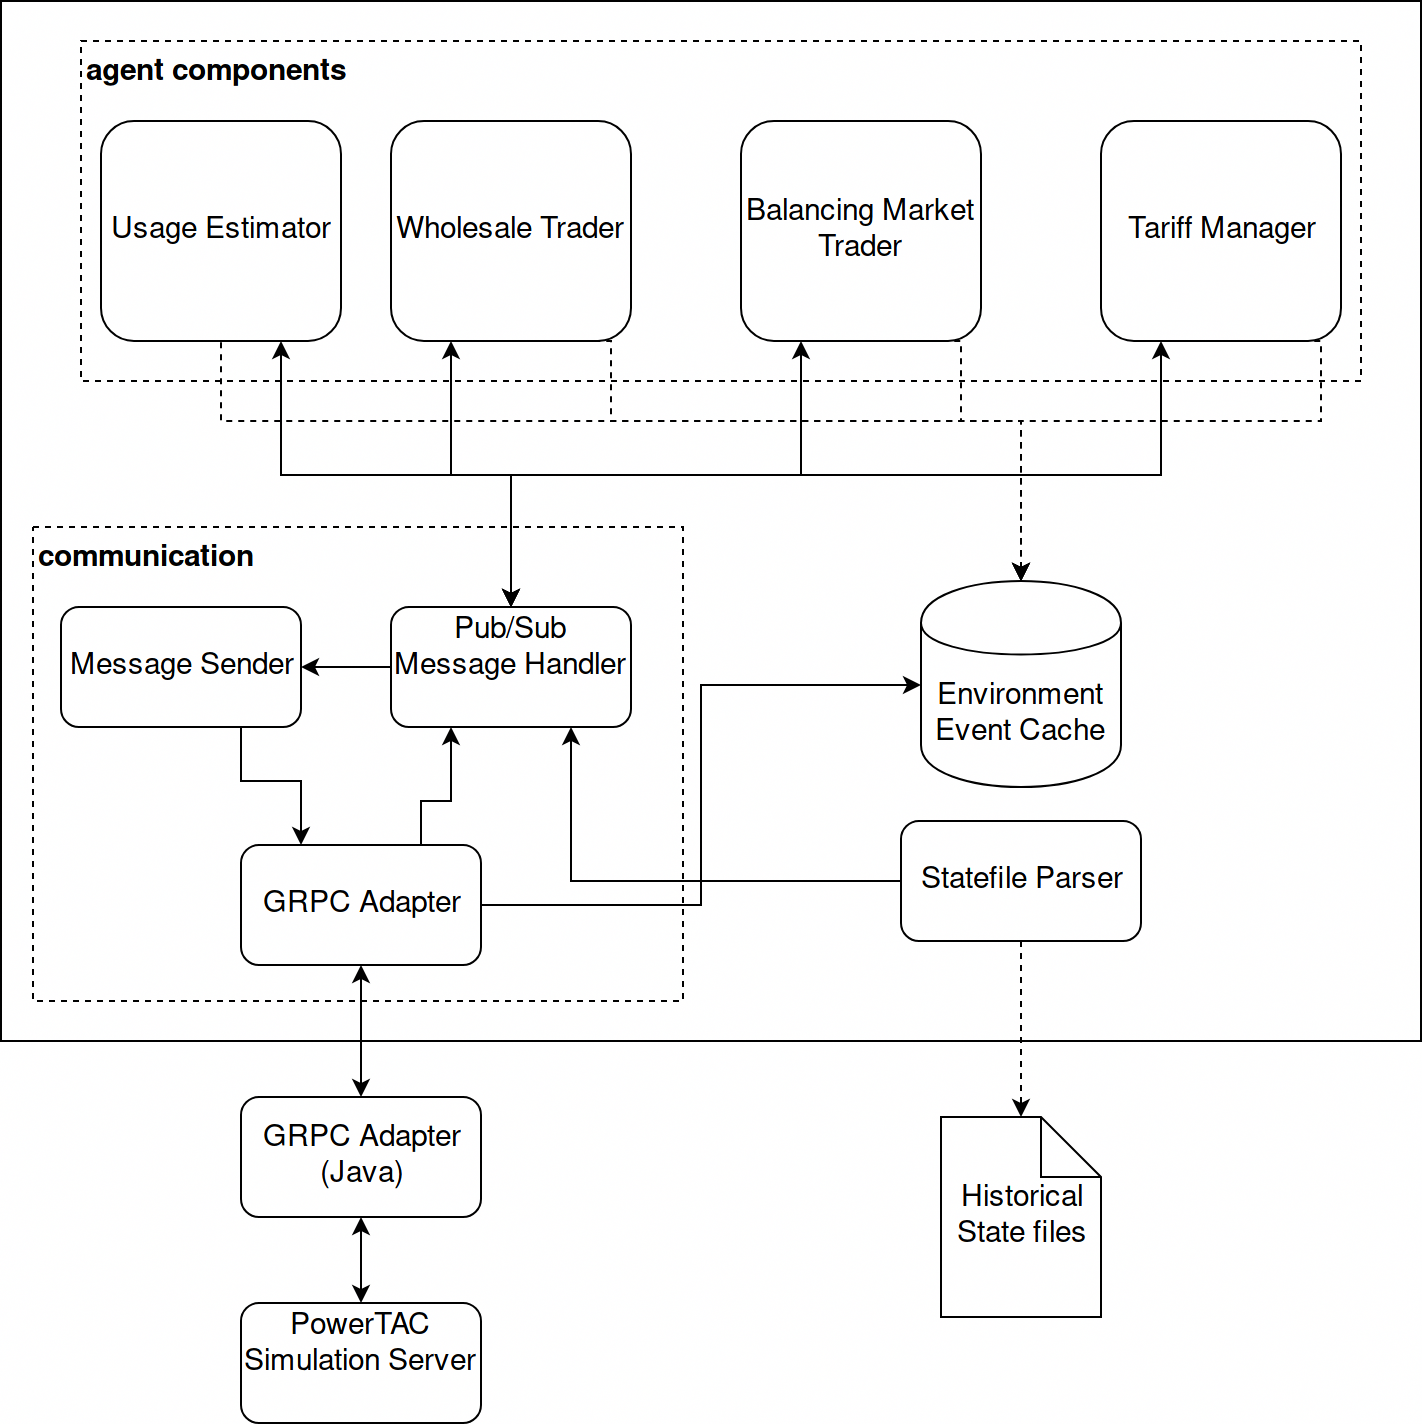
\includegraphics[width=0.8\linewidth]{img/Agent.png}
    \caption{Python Broker framework}
    \label{fig:agentframework}
\end{figure}


\section{Tools}

To develop the functionality of the agent, which is supposed to be mainly driven by deep learning technologies, a number
of state-of-the-art tools and frameworks were  used. These include
Keras and TensorFlow to allow for easy creation and adaption of the learning models,
\ac{GRPC} to communicate with the Java components of the competition and
\emph{Click} to create a CLI interface that allows the triggering of various components of the broker.

%TODO IF Kubernetes is used, I need to complete it. But what about CRIU?
%Kubernetes to easily scale several instances across the cloud.
%By transfering the components into the cloud, it is also
%possible to use tools such as Google Colab which allows access to a powerful cloud \ac{GPU} without costs
%\citep[]{GoogleColabOnline2018} .%TODO remove Google Inc in brackets


\subsection{TensorFlow and Keras}%
\label{sub:tensorflow_and_keras}

TensorFlow is a library developed by Google to facilitate machine learning algorithms. It can leverage both \ac{CPU}
and \ac{GPU} computing power which can significantly increase performance. It is Open Source, used in various
technologies and serves as a base technology for many higher level frameworks \citep{tensorflow2015-whitepaper}.

Keras is one of these higher level frameworks that focuses on \ac{NN}. It offers a intuitive \ac{API}, oriented towards
\ac{NN} terminology, to quickly develop and iterate on various \ac{NN} architectures. It integrates TensorFlow and its
accompanying UI Tensorboard, which visualizes training, network structure and activation patterns. It also supports
other base technologies beside TensorFlow, but these will not be discussed. A simple example for a 2 layer Dense \ac
{NN} written in Keras is shown in Listing~\ref{lst:kerasbasic}.


\begin{listing}
    \begin{minted}[linenos,numbersep=5pt,frame=lines,framesep=2mm]{python}
from keras.layers import Dense

model.add(Dense(units=64, activation='relu', input_dim=100))
model.add(Dense(units=10, activation='softmax'))
model.compile(loss='categorical_crossentropy',
              optimizer='sgd',
              metrics=['accuracy'])
# x_train and y_train are Numpy arrays -- just like Scikit
model.fit(x_train, y_train, epochs=5, batch_size=32)
loss_and_metrics = model.evaluate(x_test, y_test, batch_size=128)
    \end{minted}
    \caption{Basic Keras 2 layer dense NN example}
    \label{lst:kerasbasic}
\end{listing}

\subsection{Click}%
\label{sub:click}

%TODO cite only name, year missing, not correct?
Click allows the creation of CLI interfaces in Python. Programms can be customised with parameters and options as well
as structured into subcommands and groups \citep{clickcli}. This allows for patterns such as \texttt{agent compete
--continuous} or \texttt{agent learn demand --model dense --tag v2}. An annotated function is shown in
Listing~\ref{lst:click_sample}.

\begin{listing}[h]
    \begin{minted}[linenos,numbersep=5pt,frame=lines,framesep=2mm]{python}
@cli.command()
@click.option('--continuous', default=True)
def compete(continuous):
    """take part in a powertac competition"""
    import communication.powertac_communication_server as server
    server.serve()
    \end{minted}
    \caption{Click sample declaration}
    \label{lst:click_sample}
\end{listing}

\subsection{CRIU}%
\label{sub:criu}
\ac{CRIU} allows the freezing and storage of an application during runtime. This permits what is an equivalent of a fork
of the \ac{PowerTAC} simulation in a given point in time. Because \ac{CRIU} is also integrated into Docker, creating
containers for various components of the competition (i.e. server and brokers) and freezing all of them in a coordinated
manner is very helpful. This allows for two "what if" scenarios to play out at a given point in time where the results
can be compared \citep{criu}. A typical scenario for the technology is the live migration of running applications across
server infrastructures. In theory, a checkpoint of an application allows the perfect recreation of the application state
even after a complete reboot of the machine or the moving of the application to a different host with identical
environment settings.

\subsection{Docker}
\label{sub:docker}


Docker allows to create isolated, transferable images that include everything an application requires to run. A
container can be based on various distributions and many containers can run on a single server without much overhead.
\ac{VM} technologies are often compared to containers, but \ac{VM}s abstract on a different layer. A \ac{VM} simulates
an entire operating system on top of a layer called the hypervisor. Docker on the other hand only abstracts the
application layer, letting all containers run in the same kernel and therefore makes use of the existing ressources in a
more efficient way. Because \ac{CRIU} is integrated into Docker
\footnote{at the time of writing, CRIU support is experimental in Docker},
containers can be stored to disk using the \emph{checkpoint} feature.

\subsection{\ac{GRPC}}%
\label{sub:grpc}

\acf {GRPC} is a remote procedure call framework developed by Google Inc. It allows various languages and technologies to
communicate with each other through a common binary format called \emph{protocoll buffers} or short \emph{protobuf}. All communication can be encrypted via SSL, offering
security and authentication. Over-the-wire data representation can either be binary or \ac{JSON}
\citep[]{grpc}. The benefits over the
current implementation are described in Section~\ref{sub:grpc_based_communication}.


\subsection{MapStruct}%
\label{sub:mapstruct}

MapStruct offers transferring data between Java Objects of different classes. This problem is very common in large
software projects where domain objects may be out of the control of the developing team or based on external libraries.
If several components need to be integrated, translation is often necessary to adhere to the object structure required
by the library. MapStruct offers to generate otherwise manually created code based on best practices and naming
conventions. It is compile-time based, generating all code during compile time. This offers better error avoidance and
performance compared to alternatives that are reflection based
\citep[]{mapstruct}.
An example is given in Section~\ref{sub:implementing_the_communication_with_ac_grpc_and_mapstruct}.




\section{Preprocessing}
\label{sec:preprocessing}

To learn from the large amount of data already available from previous simulations, parsing the state files provided by
the simulation is a reasonable approach to boost the ability of several parts of the agent to learn faster. One example
is the predictor of customer energy usage, as previous simulations offer large amounts of usage data that can be
analyzed.

The original approach was to manually parse these files using python and to reconstruct the server state in python.
While this was successful for the demand component, I discovered the powertac-tools repository which holds similar tools
based on a combination of python and java components. This repository allows the creation of customer production and
consumption information in a comma separated file format. The initial approach to parse the files was therefore scrapped
and replaced with this prebuilt variant that makes use of the powertac-server source code.

While the current demand prediction is solely based on historical demand, this can easily extended (as it has been in
the python only approach previously mentioned) with weather data, time information and up-to-date tariff information
\footnote{All preprocessing code has been deleted in commit
    \href{https://github.com/pascalwhoop/broker-python/commit/c54ee7c05585d15462f40e2be6850343e8aea27a}{c54ee7c} in the
broker-python repository.}.


%The general architecture of the agent follows the idea of a core \emph{environment} module that holds all relevant data
%for a game. Tariffs, rates, customers, transactions and other data is stored in this module. Since the state files are
%based on events (they hold constructor parameters and method call parameters of previous server instances), these events
%need to be applied to the environment. To learn from these events, most modern frameworks require a training
%data-set and a label data-set. Therefore these events are first applied to the environment and at each time slot,
%relevant training samples are extracted. Therefore the overall structure of the translation from state files to training
%data is as follows:

%\begin{enumerate}
%    \item Iterate over all local state files
%    \item Iterate over lines in state file
%    \item Apply line to
%        current environment state
%    \item At each time slot, extract relevant samples
%    \item Store training data in separate local
%        %TODO separate vs online/streaming structured approach
%files \end{enumerate}
%
%The code linked to the process described above is part of the \texttt{util.state\_extractor} and
%\texttt{model.environment} modules. The tests in the \texttt{tests} module document the functionality.
%
%After the translation, the data is usually structured in a multi-dimensional array which can be read by numpy and
%processed with Keras. First, some preprocessing can be applied with scikit-learn to analyze the structure of the data as
%well as ensure the values that are fed to the \ac{NN} don't negatively impact the learning progress. The overall
%approach follows the recommendations of \citep{Goodfellow-et-al-2016}.


\section{Connecting Python agents to PowerTAC}%
\label{sec:connecting_python_agents_to_powertac}



To connect an agent based on Python to the \ac{PowerTAC} systems, a new adapter was developed. In early 2018, a simple bridge
was provided by John Collins, a member of the \ac{PowerTAC} team. It allowed external processes to communicate with the
system through a bridge via the provided sample-broker. All messages received by the broker were written to a First in
First Out pipe on the local file system and a second pipe was created to read messages from the external process. This
was the first approach towards opening up the simulation to other languages and development environments.


As I am interested in writing my Agent using certain frameworks which are mainly developed and maintained in Python and
because it is helpful to also allow access to the adapter via network interfaces (to allow for distributed execution of
the components in e.g. cloud or container environments), I needed to adapt this to allow network based access. In general
the following problems needed to be solved:

\begin{itemize}
    \item Java model classes should be reused if possible, automatically generating target language model
        definitions from the Java source code to avoid duplication of semantically identical information
    \item Permit future developers using even more languages (such as C, R or Go) with little effort
    \item Possibly lay the basis for a change of the communication technology of the entire simulation which is more
        language agnostic.
\end{itemize}

\subsection{Evaluating communication alternatives}%
\label{sub:evaluating_communication_alternatives}

After researching the current implementation and based on previous development experiences and current best practices,
the following three alternatives have been investigated in detail.


\subsubsection{\acs {XML} via \acs {GRPC} }%
\label{sub:xml_via_ac_grpc}


The first approach is quiet similar to the original bridge but instead of writing the \ac{XML} strings to the local file
system, they are passed to the final environment via \ac{GRPC} by simple messages that just serve as a wrapper for the
\ac{XML} string. While this is not elegant from a engineering perspective (\ac{GRPC} should be used on a method level
and messages should not contain other message formats as strings), it is simple and leads to quick results. A problem
is that the resulting \ac{XML} will then have to be parsed in the Python broker. Before the introduction of other
languages, the communication was basically an internal API and broker developers only needed to concern themselves with
the handling of the Java \texttt{handleMessage} method . Therefore, no formal descriptions for the structure of the \ac
{XML} messages exist. All \ac{XML} parsing would therefore be based on observable structures of the \ac{XML} which can
be extracted from the sample-broker logs and all model classes need to be rewritten. Furthermore, agents wanting to use
other programming languages would have to reimplement all of this again, with no reuse possible.

\subsubsection{True GRPC}%
\label{sub:grpc_based_communication}

A better but more complicated approach is based on \ac{GRPC} to transmit the messages between the Java sample-broker and
the final client, hooking into the \texttt{handleMessage} methods in the sample broker.
While previous developers have handled these messages in the Java environment, I
pass these messages to the ultimate environment by converting them into protobuf messages which are then sent to a
connected broker who implements corresponding handler methods in the target language.

The advantage of this approach is
that this theoretically allows the maintainers of the project to also adapt this approach for the Java clients in
general, massively reducing the communication overhead of \ac{XML} messages. The over-the-wire protocol is much more
efficient (as the data is sent in a binary format) and the message structure is clearly documented in the
\texttt{grpc\_messages.proto} file. When serializing a \texttt{Competition} object, \ac{XML} requires 48 kByte while
the protobuf message is 14 kByte large, 70\% smaller.
\footnote{\url{https://github.com/pascalwhoop/grpc-adapter/blob/master/adapter/src/test/java/org/powertac/grpc/mappers/CompetitionMapperTest.java#L64}}.
When looking at the serialization and deserialization performance of \ac{XML} vs protobufs, a comparison of 1000
iterations of each operation for each variant also shows a significant improvement. While the deserialization of
protobuf messages performs about 5x less well (7444ms protobufs, 1366ms \ac{XML}), the serialization is 44x times
faster (1619ms \ac{XML}, 37ms protobufs)
\footnote{\url{https://github.com/pascalwhoop/grpc-adapter/blob/master/adapter/src/test/java/org/powertac/grpc/mappers/CompetitionMapperTest.java#L90}}.
This can be explained by the amount of string handling that \ac{XML} requires and on the other hand the fact that the
deserialization of protobuf messages includes a mapping of the binary format into the proper Java object via MapStruct instead
of using reflection. Generally, the server sends more messages than it receives, having to answer most messages and
redistribute information to all participants for any public information.


The disadvantage is the need to translate each \ac{POJO} into a protobuf message and
vice versa. This is however not different from the current XStream implementation which also requires the annotation of
class files in Java to declare which properties are serialized and included in the \ac{XML} strings. If the project
should adopt the \ac{GRPC} based communication, the \ac{GRPC} architecture will then allow the server to be addressed by
any of the supported languages \footnote{Which as of today are: C++, Java, Python, Go, Ruby, C\#, Node.js, PHP and
Dart}. Using MapStruct as a mapping tool also makes the mapping structured and by performing roundtrip tests of the
transformed elements, it can be assured that the transformations between protobuf messages and \ac{POJO} perform as expected
\footnote{\url{https://github.com/pascalwhoop/grpc-adapter/blob/master/adapter/src/test/java/org/powertac/grpc/mappers/AbstractMapperTest.java#L54}}.



\subsubsection{JSON schema based communication}%
\label{sub:json_schema_based_communication}


A final approach is the generation of schema definitions from the Java model classes that are transmitted between the
brokers and the server. This formalizes the currently informal \ac{XML} \ac{API}. Generally, two human readable over-the-wire structures are reasonable: \ac{XML} and \ac{JSON}.
\ac{XML} messages can be formally defined using \ac{XML} Schemas and the \ac{JAXB} project
\footnote{\url{https://github.com/javaee/jaxb-v2}} offers to generate such schemas from Java class definitions. This
however did not succeed for the \ac{PowerTAC} model definitions which lead me to create a question on StackOverflow, a
discussion platform for programming questions. The resulting answer lead to the ultimate alternative which is the
generation of \ac{JSON} schemas which can then be converted into Python class files
\footnote{\url{https://stackoverflow.com/questions/49630662/convert-java-class-structures-to-python-classes/49777613\#49777613}}.
The choice of \ac{JSON} as the base communication protocol might also be intelligent as a future choice two reasons:
Firstly, it seems to be the more popular serialization protocol in comparison to \ac{XML} \citep{jsonxml} due to its
easy readability and because it is more data efficient. Secondly, \ac{GRPC} can also transmit data in \ac{JSON} form
and protobuf messages can easily be printed as \ac{JSON}, making both alternatives more interoperable
\footnote{\url{https://github.com/powertac/broker-adapter-grpc} }.

%Because the programming language is different from the supplied sample-broker, many of the domain objects need to be
%redefined and some code redeveloped. The classes in \ac{PowerTAC} which are transferred between the client and the
%server are all annotated so that the \ac{XML} serializer can translate between the \ac{XML}  and object variants without errors.
%This helps to recreate a similar functionality for the needed classes in the python environment. If the project was
%started again today, it might have been simpler to first define a set of message types in a language such as Protocol
%Buffers, the underlying technology of \ac{GRPC}, but because all current systems rely on \ac{JMI} communication, it is
%better to manually recreate these translators. The \ac{XML} parsing libraries provided by Python can be used to parse
%the \ac{XML} that is received.

\subsection{Implementing the communication with \ac{GRPC} and MapStruct}%
\label{sub:implementing_the_communication_with_ac_grpc_and_mapstruct}

After adapting the projects scope in response to the mid-thesis coordination with my supervisor, I chose the second
approach, the pure \ac{GRPC} solution. Because the focus will now be on the wholesale market, only a subset of messages
need to be mapped. This permits the implementation of a subset of message mappers between the protobuf and
\ac{PowerTAC} entities, reducing the scope while retaining the benefits of a \ac{GRPC} implementation which generally
can be regarded as the best alternative.

Using MapStruct, all messages required for the wholesale learning component are mapped from the simulation core entities
to the protobuf messages. To map classes, a mapper interface is created for each type. Most simple types can
automatically be mapped and don't require any adaption. All properties have been named the exact same way as the
properties of the data holding entities in the \ac{PowerTAC} environment, allowing MapStruct to deduce the
corresponding properties to map to. Some properties require custom initiation, more specifically those where the \ac
{PowerTAC} entities don't follow the bean specification for getters and setters. An example is given in
Listing~\ref{lst:mapperexample}. Mappings are defined with the \texttt{@Mappings(\{\})} annotation. Complex compositing
objects require the other needed Mappers to be defined in the \texttt{@Mapper(uses = \{...\})} annotation. Support for
protocol buffers in MapStruct is still fresh and many currently required lines of code may soon be redundant.

To ensure the mapping works as expected, the tests for the mapper classes perform a \emph{roundtrip test}. This takes a
Java class as commonly found in the simulation, converts it into \ac{XML} using the current XStream systems, then
performs a translation into protobuf  and back. Finally, this resulting object is serialized into \ac{XML} again and
both \ac{XML} strings are asserted to be equal. By doing this, many things, several things are tested at once: Is the
translation working as expected, i.e. does it retain all information of the original objects? Is the mapping of IDs to
objects still working as expected? Are any values such as dates or time values misrepresented? The roundtrip test allows
for a generic testing of all object types that covers a large number of possible errors.

\begin{listing}[]
    \begin{minted}[linenos,numbersep=5pt,frame=lines,framesep=2mm]{java}
@Mapper(uses = {
    OrderbookMapper.BuilderFactory.class,
    InstantMapper.class,
    TimeslotMapper.class,
    OrderbookOrderMapper.class

},
    collectionMappingStrategy =
        CollectionMappingStrategy.ADDER_PREFERRED,
    nullValueCheckStrategy = ALWAYS)
public interface OrderbookMapper
    extends AbstractPbPtacMapper<PBOrderbook, Orderbook>
{

  OrderbookMapper INSTANCE =
    Mappers.getMapper(OrderbookMapper.class);

  @Mappings({})
  PBOrderbook.Builder map(Orderbook in);
  @Mappings({})
  Orderbook map(PBOrderbook in, @MappingTarget Orderbook out);

  //BuilderFactory helper class
}
    \end{minted}
    \caption{Mapper for Orderbook class}
    \label{lst:mapperexample}
\end{listing}

With an ability to translate Java objects into protobuf messages, those messages now need to be transferred. \ac{GRPC}
offers the ability to transfer protocol buffer objects both as streams and as unary operations. The entire communication
overhead between the server and the client is abstracted away from the developer. The messages can therefore simply be
sent to the connected python broker code through the \ac{GRPC} adapter. The integration with the existing code is shown
in Listing~\ref{lst:handlemessageexample}.

\begin{listing}
    \begin{minted}[linenos,numbersep=5pt,frame=lines,framesep=2mm]{java}
public synchronized void handleMessage(Orderbook orderbook)
  {
    PBOrderbook msg = comm.converter.convert(orderbook);
    comm.marketStub.handlePBOrderbook(msg);
  }
    \end{minted}
    \caption{handleMessage example}
    \label{lst:handlemessageexample}
\end{listing}

On the Python side, the messages are now accepted and applied to the brokers knowledge base. This is encapsulated in the
env module of the broker as described before. Some messages may also be considered as action triggers and are therefore
shared with all interested components through the publish-subscribe event system. A message signaling a completed
time slot for example may trigger the broker to learn on the newly observed usage patterns, improve its predictions on
the expected usages of its customers and evaluate its next steps in the wholesale trading market. To perform such
actions however, the broker must first be able to compete in a competition.

\section{Creating Containers from competition components}
\label{sec:creating_containers_from_competition_components}

To run a competition on a local machine, one must install several components: Maven, Java 8 and all of the brokers as
well as ones own technology stack. If the scale of this set of components exceeds the local computation power available,
the stack needs to be moved to a machine in a server with sufficient computation power. While tools like Vagrant allow
the configuration and setup of environments to quickly allow new developers to start working with a set of tools in a
given project \citep{vagrant} , it requires virtual machines which have significant overhead in comparison to container
technologies. If the competition is abstracted into docker images, tools like Kubernetes or Docker Compose can quickly
instantiate a competition on any machine, given it has enough resources and a docker runtime installed \citep{docker}.
Containerized application infrastructures have recently become quiet popular. Amazon, Google and Microsoft are offering
services specifically tailored to host containerized applications and it is quiet easy to share created docker images
through the docker hub platform.

To create a Docker image for the server, the \texttt{Dockerfile} listed in Listing~\ref{lst:servertodocker} can be used
\footnote{All resources regarding the container technologies can be found under
\url{https://github.com/pascalwhoop/powertac-kubernetes}}.
It is also common practice to run the build in one container and move the created executable artifact into another
container that is solely responsible for executing said artifact. The \emph{alpine} image type is an extremely
light-weight Linux base that only requires about 5Mb of storage. Container images are therefore quiet light-weight in comparison
to virtual machines.

\begin{listing}[h]

    \begin{minted}[linenos,numbersep=5pt,frame=lines,framesep=2mm]{Dockerfile}
FROM openjdk:alpine
LABEL maintainer=pascalwhoop
LABEL name=powertac-server

WORKDIR /powertac
RUN mkdir data

COPY bootstrap-data.xml ./
COPY init.sh ./
COPY server.properties ./
#assumes a built server jar is present in the target folder
COPY target/server-jar-1.5.1-SNAPSHOT.jar server.jar

EXPOSE 8080 61616
#and start it up
CMD "/powertac/init.sh"
    \end{minted}
    \caption{Turning the current server snapshot into a docker image}
    \label{lst:servertodocker}
\end{listing}

This offers another advantage that may become increasingly attractive in the long-term: Tools like Kubernetes or Docker Swarm, both being open source enterprise level container management
software, seamlessly allow for the creation of 1, 10 or 1000 instances. OpenAI, a deep learning research company, has
successfully scaled Kubernetes to 2500 nodes to run their deep \ac{RL} learning systems \citep{openai2500}. As
previously mentioned, Docker also integrates \ac{CRIU} which is required for the creation of snapshots of competition
states.

%TODO implement redis as base for communication between components
%\subsection{Redis and component messaging}%
%\label{sub:redis_and_messaging}

\section{Inner Python communication}%
\label{sub:inner_python_communication}

Once the competition environment is running and messages start streaming into the python environment, the various
components need to be coordinated in an intelligent fashion. Event driven architectures are light-weight and offer
enough flexibility to coordinate the various components. The server may send a number of \texttt{TariffTransaction}
messages followed by a \texttt{TimeslotComplete} message that signals the demand estimator it may now calculate new
forecasts for any customer subscribed to the broker. Once the component has completed the task, instead of directly
calling another component such as the wholesale trader, it sends a signal via the event system so that any subscribed
component may react to the event. Because the simulation only accepts messages within a certain time-frame, tardy
messages are ignored. Components need to observe the message topics of interest to them and start their processing as
soon as they have collected all the necessary information.

To enable possible later extensions to also access events retrospectively, all events are cached in an in-memory event
store. If the event load becomes too large to fit into memory, this may be outsourced into a file-system backed caching
mechanism.

%The components of the agent that have learning capabilities include:
%
%\begin{description}
%    %TODO will i still get to implement this? simply mimick an agents tariffs ... shouldn't be hard. The default tariff
%    %is already sent to the server from within Java, so that is also an option.
%    \item[Customer Market]: Generates actions in respect to the tariff market such as publishing,
%        adapting and revoking tariffs. While the component is expected to have a positive impact on the performance of
%        the broker, it was just implemented with a basic functionality of publishing the same tariffs as a selected
%        competitive broker, mimicking the competing brokers portfolio. It also creates usage predictions for a set of
%        customers for other components. Generally, the framework intends a tariff fitness evaluation as well as tariff
%        selection component that weighs both competitiveness and expected profitability.
%
%    \item[Wholesale Market]: Places bids and asks for energy in the periodic double
%        auction type market \citep{ketter2018powertac}. The component employs \ac{RL} techniques and uses the
%        predictions generated from the customer market component as an input describing the required capacity.
%
%    \item[Balancing Market]: The balancing market component has not been implemented, but it is part of the
%developed framework for possible future extension.  \end{description}

\section{Usage Estimator}
\label{sec:usage_estimator}

%The customer market component covers the tariff market and the demand prediction tasks. In my implementation, the
%broker does not perform autonomous tariff creation but instead just publishes the default tariffs. The goal was to focus
%on the wholesale market and the demand prediction.


%TODO background?
%TODO not implemented
%The goal of the customer market is to get as many subscribers as possible for the most profitable tariffs the broker
%offers on the market. The tariffs offered in the market compete for the limited number of customers available and every
%customer must be subscribed to some tariff. The profitability of tariffs is limited by the base tariff which is offered
%by the simulation as a constant offering creating an upper bound on profitability.
%
%To succeed in the customer market, the agents needs to be able to generate tariffs that are competitive. This can be
%broken down into two subtasks: Generating valid tariffs and evaluating their competitiveness. A tariff can be verified
%by passing it to the \ac{PowerTAC} server which verifies the tariff. Hence, a \ac{RL} algorithm that is tasked with
%creating competitive tariffs can be given feedback by penalizing non-conclusive tariffs. An invalid tariff could be one
%that contains overlapping rates leading to an ambivalent status. The competitiveness of a tariff depends not only on the
%attributes of the tariff but also on the competition environment. If the broker only competes against the default
%tariffs, even many mediocre tariff offerings would perform well. In an environment with many competitors on the other
%hand, a tariff needs to be well designed to generate profits.
%
%The agents learning task for the customer market is therefore designed in the following way:
%
%\begin{enumerate} \item Learning to evaluate a tariffs competitiveness in relation to the competitive environment
%   through supervised learning on the historical state logs of previous competitions \item Running a \ac{RL}
%   algorithm which learns to choose parameters for tariffs that are valid and profitable in a given environment
%    %\item Learning to generate valid tariff specifications through a genetic algorithm strategy, penalizing invalid
%   %tariffs %TODO really, I go genetic?
%\end{enumerate}
%
%%TODO not yet actually realized, still applicable?
%\subsubsection{Tariff fitness learning} To learn the fitness of a tariff while considering its environment, supervised
%learning techniques can be applied. To do this, features need to be created from the tariffs specifications and its
%competitive environment. Similar work has been done by \citep{cuevas2015distributed} who discretized the tariff market
%in four variables describing the relationships between the competitors and their broker.
%
%For my broker, because \ac{NN} can handle a large state spaces, I create a more detailed description of the
%environment. I still have to ensure the number of input features is fixed though, so a simple copy of all competing
%tariffs is not a valid input for the environment description. Instead I create the following features from the tariff
%market:
%
%\begin{description} \item[Average Charge per hour of week Timeslot]: According to \\
%   \texttt{TariffEvaluationHelper.java}, customer models evaluate tariffs on an per-hour basis. This means they are
%   very precise in the evaluation of potential tariff alternatives (before the application of an irrationality
%   factor). Hence, a per-hour precision in the input is needed.  \item[Variance of Charge per hour of week
%   Timeslot] Variance of the tariffs charges per each time slot in a week among all competitors.  \item[Average and
%   Variance of periodic payments] Description of the markets periodic payments landscape \item[Average and Variance
%   of one-time payments] Description of the markets one-time payments landscape \item[Average and Variance of
%   Up/Down regulation payments] 0 for tariffs without regulation capabilities \end{description}
%
%Because the \ac{PowerTAC} simulation does not return profits of brokers on a per-tariff basis and because the reasons
%for why a broker purchased a specific amount of energy on the wholesale market are not known, it is hard to put a
%profitability value on a brokers tariff if said broker offers more than one tariff on the market. Therefore the
%evaluation of the tariff does not include the profitability of the tariff but merely the competitiveness in regards to
%the attractiveness of the offer from the perspective of the customers
% large space of decision variables / dimensions
%
% how to avoid overwhelming of agent? output layer must be fairly large.
%
% time, energy, money, communication dimensions (and subdimensions)

%\subsection{Customer demand estimation}% \label{ssub:customer_demand_estimation}
%\label{sub:customer_demand_estimation}

The broker needs to predict the amount of energy the customers in its portfolio will require to make good decisions in
the wholesale market.
When predicting demand, it is helpful to first perform a preliminary analysis of the structure of the demand patterns.
This has been done using Jupyter Notebooks and the work can be seen in the \texttt{notebooks} folder in the
broker-python code repository
\footnote{\url{https://github.com/pascalwhoop/broker-python/blob/master/notebooks}}. All data was generated using the
\texttt{powertac-tools} project. Generally, the customer patterns
vary widely and it is quiet difficult to predict individual customer usage. When the number of customers increases
though, the individual errors partially cancel each other out and the overall predictability increases.
Figure~\ref{fig:demandtimelag} shows a clear correlation between the current demand of the market and historical demands with a
delay of 12,24,36,48,... hours. This correlation degrades and slowly converges towards no correlation.

\begin{figure}[]
    \centering
    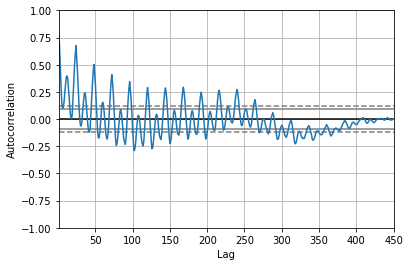
\includegraphics[width=0.6\linewidth]{img/demand_6.png}
    \caption{Lag Plot showing the correlation of the population usage data in relation to the time lag}
    \label{fig:demandtimelag}
\end{figure}

The analysis also showed large differences in the demand profile of different customers. Some consume several thousand
\ac{mWh} per time slot while most normal consumers only consume small amounts. This however is not directly
translatable into tariff market actions because some customers are actually just a population model that simulates many
thousand individuals. These models may create contracts with a number of brokers, breaking the demand of these large
models down into several small transactions spread across tariffs.

From a technical perspective, this component has no dependencies onto the other learning components and can easily be
trained using historical data. It is therefore a supervised learning algorithm, matching known information in time slot
$t-n$ to a prediction for the expected energy usage at time slot $t$. Because there are several games on record, the
historical realized usages are the labels for the supervised learning problem. Known information includes: Weather
forecasts, historical usages, time, tariff and customer metadata. A simplest approach and therefore a baseline to
measure against is to predict the customer to consume the same amount as in the previous time slot. All demand
prediction loss is measured in mean average error. A linear error is chosen because the economic impact of misjudging a
demand is also linear. When using such a prediction method as well as a -12h and -24h prediction, the results are as
seen in Figure~\ref{fig:demand_baseline}.

\begin{figure}[]
    \centering
    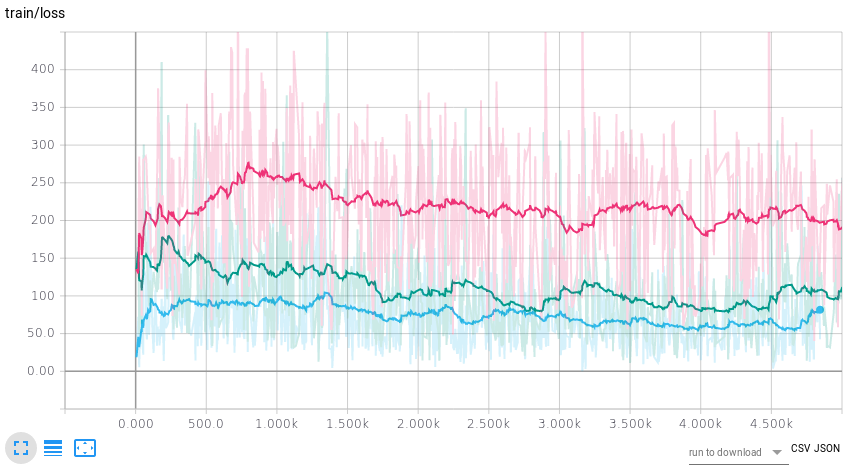
\includegraphics[width=0.8\linewidth]{img/demand_baselines.png}
    \caption{Demand baselines, -1h blue, -12h pink, -24h green}
    \label{fig:demand_baseline}
\end{figure}

%A random prediction based on a neural network being fed random data usually
%levels out at 300 to 400. This gives a goal range (below -24h prediction) as well as a pattern to avoid which
%basically equals not learning anything.
Several architectures were tried, however none significantly outperformed a simple heuristic approach such as guessing
the demand to be equivalent to that of 24 hours ago. A later analysis
\footnote{see jupyter notebook "Trying various forms of Demand Models on single customers.ipynb"}
revealed why this occurs. The neural networks architectures are having trouble handling both very large and very small
customer patterns. When training a neural network for each customer individually, the performance is much higher. This
intuitively leads to the idea that creating a model for each customer may lead to a performance boost. This however
creates a range of other complications. Most frameworks are written based on the assumption that one neural network is
trained per machine. Most neural networks are only limited by the amount of hardware that is available as well as the
data that it may learn from. Having some 200+ neural networks learning from data and predicting in parallel, all in
under 5 seconds per time slot is hard to achieve on conventional hardware. A test run showed that the system can only
process one customer every 3 seconds. While this does include the creation, compilation and fitting of the model, it is
near impossible to reduce
this number enough to be able to handle all customers within the initial 5 seconds of the game. It was therefore
necessary to either add significant amount of processing power to the broker or somehow get one model to predict all
kinds of customer classes with decent precision. One improvement was the creation of a separate preprocessing scaler for
each customer. While the previous approach used one \texttt{MinMaxScaler}, a scaler that scales all values between two
limits, usually 0 and 1, the second approach was the creation of a scaler for each customer, to allow for a individual
scaling across customers. The difference is visualized in Figure~\ref{fig:imgfrosty}

\begin{figure}[]
    \centering
    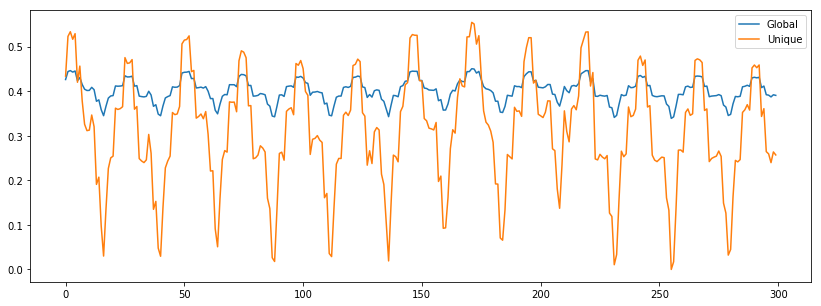
\includegraphics[width=0.8\linewidth]{img/frosty_scaled.png}
    \caption{Scaled as game (yellow)  or individually (blue)}
    \label{fig:imgfrosty}
\end{figure}

Ultimately, the predictor model that seemed most successful in terms of average error and robustness against repetitive
training against various types of usage patterns was a dense vanilla feed-forward \ac{NN} with
\texttt{168,100,100,50,50,24} units, using stochastic gradient descent as its optimization function and mostly using
\ac{ReLu} activation function except for the last layer which is a linear activation. To overcome the problem of
catastrophic forgetting, a common phenomenon observed when networks have been trained on several tasks in sequence
\cite[]{french1999catastrophic}, all input data is shuffled instead of processed in sequence per customer. While this
does not keep the network from forgetting, it makes it forget learned knowledge about patterns uniformly, replacing the
previous weights with newly learned weights from newly observed patterns uniformly. Results for this predictor are shown
in Figure~\ref{fig:imgcombined_model}, a comparison with the baseline and more examples of various customer types of
-24h are given in the appendix. It is clearly visible from the figure that the model has learned to predict regular
spikes. It doesn't seem to understand that there is a natural maximum to the usage pattern, which is understandable for
a continuous model. It also doesn't quiet capture the reduced usage on everry 7th day as can be seen via the flat hump
in the brown realized curve. 
%TODO appendix number of figure

The timing of this unified model is also acceptable with 3 to 4 ms per 24h forecast required, adding up to a 800 ms
delay for predicting 200 customers, which would almost cover the entire games customer base.

\begin{figure}
    \centering
    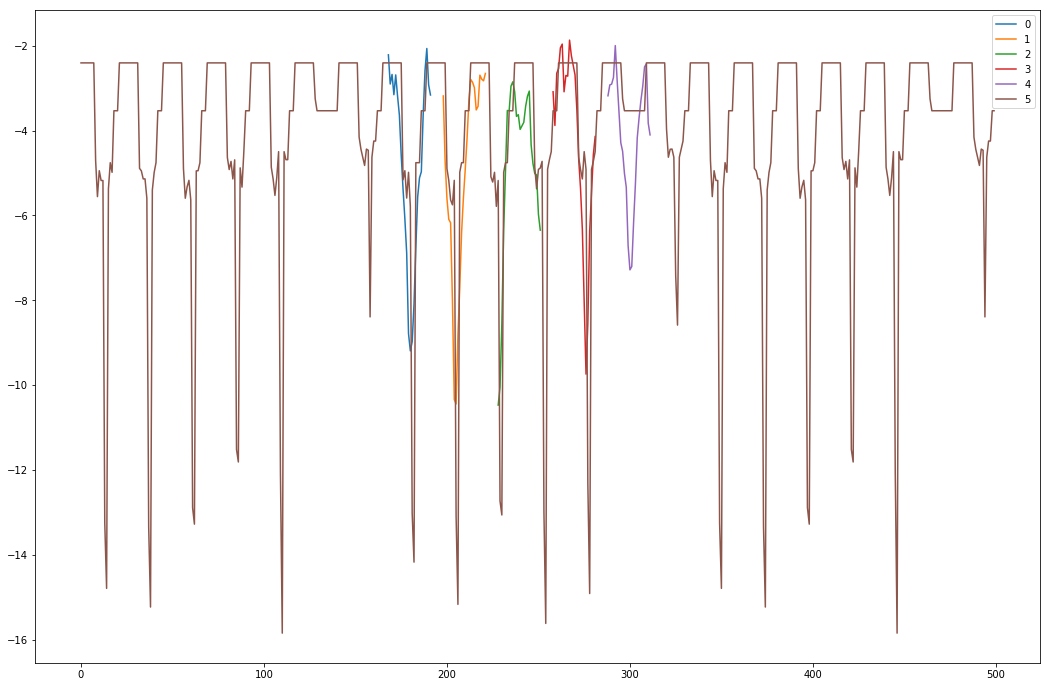
\includegraphics[width =0.8\linewidth]{img/pred1.png}}
    \caption{Plotting of forecasts and realized usage}
    \label{fig:imgcombined_model}
\end{figure}



%If the customer models change across games (e.g. if a customer suddenly uses 10x the energy on rainy days), the learning
%model will have to learn to adapt to this change. This can be achieved by letting the model both learn from historical
%data initially (i.e. form the state files) and also let it learn online during the competition, based on the new
%customer models.
%
%To train a model that predicts the demand amounts of customers under various conditions, a dataset of features and
%labels needs to be created. Because the model may also learn during the course of a running competition, a generator
%based structure should be preferred. This means that a generator exists that creates $x, y$ pairs for the model to train
%on, instead of creating a large batch of learning data ahead of the learning processing, which is otherwise a common
%practice. Whenever a round completes and new information is available, the demand estimator is asked to estimate the
%demand for all customers subscribed to the tariffs of the broker for the next 24 time slots. These estimations are then
%saved (i.e. they replace any previous estimations) and the wholesale component as well as other components can act on
%this newly created estimations.

%According to the simulation specification, the customer models generate their demand pattern based on their internal
%structure, broker factors and game factors \citep[]{ketter2018powertac}. The preprocessing pipeline of the generator therefore generates
%feature-label pairs that include: Customer, tariff, weather, time and demand information. The realized demand is the
%label while all other components are part of the features that are used to train the model. The intuitive model class
%for demand patterns prediction are \ac{RNN} due to the sequential nature of the problem \citep[]{EvalGRU2014}. However,
%as will be shown later, the implementation of relatively shallow dense classic \ac{NN} also results in decent results.

\begin{figure}[h]
    %TODO export new variant in drawio
    \centering
    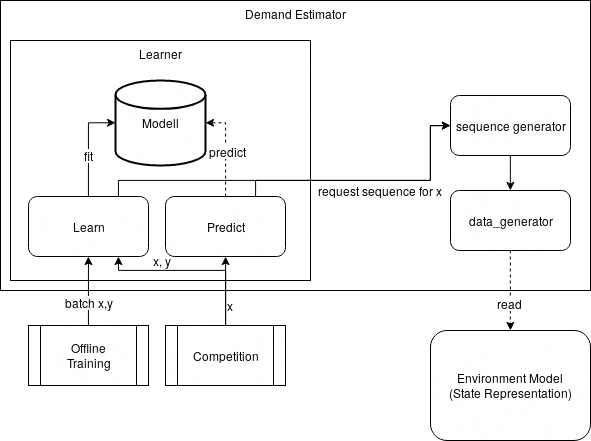
\includegraphics[width=0.8\linewidth]{img/UsageEstimator.png}
    \caption{Demand Estimator structure}
    \label{fig:DemandEstimator}
\end{figure}

Once the general concept of the learning model was decent, a surrounding architecture had to be built to allow this
network to both learn and predict live in a game setting.
The overall structure of the demand estimator component is shown in Figure~\ref{fig:DemandEstimator}. The model can be
both trained offline based on the state files as well as online during the competition. This is possible because in both
situations, the environment model of the agent is a continuous representation of the agents knowledge about the world.
In fact, during the state file parsing, the environment may even hold information that the agent usually cannot observe
in a competition environment. This is also the case for the demand learning, as the state files hold the demand
realizations of all customers while the server during the competition only transmits the usage realizations of the
customers that are subscribed to the agents tariffs. Regardless, this does not affect the ability to learn from the
customers usage patterns in either setting. During a competition, the agent may learn from the realized usage of
customers after each time slot is completed. Because this process may require some resources, it is advantageous to
first perform the prediction of the subscribed customers demands for the current time slot to pass this information to
the wholesale component before training the model on the received meter readings. While the broker is waiting for the
server to process a step in the game, it can perform any learning on newly received information \footnote{The component code can be
found under \url{https://github.com/pascalwhoop/broker-python/tree/master/agent_components/demand}}.

%TODO write final model structure and plot against intuitive -24h baselines

\section{Wholesale Market}
\label{sec:wholesale_market}

To approach the wholesale trading problem, a subset of the definition of the trading problem developed by
\citet{tactexurieli2016mdp} is assumed. More specifically, the agent only concerns itself with the activities in the
wholesale market and does not act or evaluate tariff market or balancing market activities.

They defined each of the target time slots as a \ac{MDP} with 24 states before termination. Termination occurs when
there are no further trading opportunities for a time slot and the \ac{DU} applies the final balancing fee to the
time slot. Brokers that have predicted their usage precisely and traded matching amounts of energy in the wholesale
market require less balancing than those that either suffer bad forecasting or are not capable to place orders
successfully before the trading is closed. The reward function may be composed in different ways but the most generic
consideration is the profit achieved by the broker for the given time slot. Because this reward design suffers strong
noise from the market price fluctuations, different reward functions may be preferred as discussed later.

An alternative approach for modeling the wholesale market would be to consider the entire game a single \ac{MDP} where
the agent has to make 24 decisions per slot and receives rewards each step for the completed slot. The environment would not involve a
\emph{reset} event, because the environment would never be reset. The entire game would be one long episode.

Both approaches have advantages and disadvantages. The former creates short, fixed-length episodes that more closely
match the concepts of contemporary \ac{RL} problems such as the locomotion examples described in
Chapter~\ref{cha:background}. However, because \ac{PowerTAC} allows for trading up to 24 hours into the future, 24
environments would have to be stepped in parallel. Approaches for parallel asynchronous stepping of multiple
environments with a \ac{NN} based policy function approximator exist (see \citet{mnih2016asynchronous,hafner2017agents})
but require more complex architectures that update a central policy function based on experiences from all environments.
The latter avoids this, allowing a fairly simple off-the-shelf algorithm to be applied to the problem. Problems appear
with the compatibility to the action spaces this agent requires as well as the increased signal noise. Common algorithms
such as \ac{DQN}, \ac{SARSA} or \ac{A3C} are not easily applied to such large action spaces. They
are written to be applied to discrete action spaces
\cite[]{baselines}. \ac{PowerTAC} trading is in its purest form a
continuous action space, allowing the agent to define both amount and price for a target time slot. Furthermore, the
agent would observe 24 environments in parallel, largely hindering learning performance. The network would have to learn
to match each input block to an output action, as the input for time slot 370 has little effect on the action that
should be taken in time slot 380. In a separated \ac{MDP}, each environment observation would only hold the data needed
for the specific time slot rather than information about earlier and later slots as well.

\subsection{Learning from historical data}%
\label{sub:learning_from_historical_data}

Learning quickly from historical data may be facilitated for off-policy algorithms that can learn from historical
records of other agents or, if the approach introduced in
Section~\ref{ssub:offline_record_based_wholesale_environment_approximation} is applied, also for on-policy algorithms.
To allow reuse of existing algorithm implementations, I wrote the \texttt{PowerTacLogsMDPEnvironment.py} class which
implements the \ac{API} proposed by the OpenAI gym project \cite[]{brockman2016openai}. It iterates over the existing
game logs and generates both a forecast for the \ac{RL} agent as well as some historical market data. Each time slot is
processed sequentially, before the next is started. The process is therefore changed from the competitions 24 parallel
trades paradigm to 24 sequential trades for ts $x$ followed by 24 trades for ts $x+1$. For each step per episode, an
observation is created from the historical trade data as well as the current forecast and returned to the agent. It
in return is answered by the agent with a call to \texttt{step} which is passed an action. The action is mapped to
real-world \ac{mWh} and price per \ac{mWh} amounts and evaluated. If the action would result in a clearing in the
recorded market prices (i.e. if the agent offered cheap energy or bought for a high bid), the action gets logged as a
purchase. Once the target time slot trading is completed, the reward is calculated, the environment is reset and the
next time stop is traded. The high-level flow is depicted in Figure~\ref{fig:img/WholesaleEnvironment}

\begin{figure}[]
    \centering
    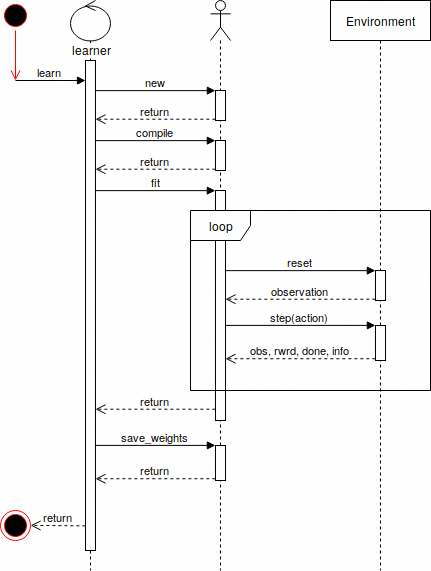
\includegraphics[width=0.6\linewidth]{img/WholesaleEnvironment.png}
    \caption{img/WholesaleEnvironment}
    \label{fig:img/WholesaleEnvironment}
\end{figure}



%As previously mentioned, \citet{tactexurieli2016mdp} define the entire simulation as a unified \ac{MDP}.
% each time slot is not considered an independent \ac{MDP} anymore!
The reward for the agent is received at the terminal state and is defined as the relation of the average price paid per
\ac{kWh} by the agent in relation to the average market \ac{kWh} price for a given time slot. This removes any bias in
the reward introduced by market price fluctuations. To calculate the reward, I first calculate the average price paid by
the agent per \ac{kWh} based on the realized price and quantity $P^r_i$ and $Q^r_i$ respectively:

\begin{equation}
    \label{eq:Average price per kWh for a given target time slot}
    %average price paid per \ac{kWh} by broker
    P^{r}_{avg} =\frac{\sum ^{1}_{i=24} P^{r}_{i} *Q^{r}_{i}}{\sum ^{1}_{i=24} Q^{r}_{i}}

    %TODO encouraging for exploration injecting into rewards

\end{equation}
This is also calculated for the market prices $P^m_{i}$ and quantities $Q^m_i$ cleared during each time slot for the whole market and then the
relationship between the agents average costs and the average market costs is used as the reward
\begin{equation}
    %relationship between average price paid by broker and average market price for target time slot
    R(t) = \frac{P^r_{avg}}{P^m_{avg}}
\end{equation}

\begin{markdown}

    ### WIP

    - adapting the wholesale environment to be  compatible to the OpenAI Gym "Environment" which allows for

\end{markdown}


Using \ac{MDP}

\ac{MDP} is actually with infinite states but for analytical concept, its irrelevant. Important is: Continuous states,
continuous actions (with some rounding to nearest .02)

Bellman equation not applicable to continuous spaces. But it is also unique because its a directed acyclic graph (the
state transition graph) 1, 2, 3, 4, ... 24

theoretically it's a nonstationary \ac{MDP} because it's limited to 24 state transitions before termination (t-0)

DQN --> evaluate the value of a s,a pair

\ac{PPO} --> use DNN for determining what to do in a given state - maximizes "surrogate" (relation between old and new
policy) while penalizing too extensive reward estimations (to avoid extensive updates to policy)

reward is based on relative price paid in comparison to average price for given time slot.

Do I implement the env interface defined by OpenAI and let the agent subcomponent imagine it's by itself? --> allows for
A3C and many other interesting opportunities

- having issues with learning the whole thing. No learning can be observed. Network output just bounces forth and back
between -1 and 1. 'tanh' activation functions used --> explains the bouncing limits. something inside of the network
makes it bounce so strongly.

%NOTES AFTER IMPROVING ON DEMAND PREDICTOR

- need to solve the multiple \ac{MDP} for one agent problem
- no off the shelf algorithms that do continuous multi agent mdp stuff
- applying \ac{NAF} / \ac{DDPG} to problem possible. But may need to rewrite \ac{NAF} agent myself. Take stuff from
Keras though. 
- doing a simple "always order demand prediction" baseline should be helpful
\chapter{Results}

\section{Demand Estimator}%
\label{sec:demand_estimator}

\section{Wholesale Market}%
\label{sec:wholesale_market}

\chapter{Conclusion}%
\label{cha:conclusion}

